\documentclass[anonymous]{lipics-v2021}
\usepackage{amsthm}

\usepackage{booktabs}
\usepackage[table]{xcolor}
\usepackage{pgfplots}
\pgfplotsset{compat=1.18}
%\usepackage{subcaption}
\usepackage{graphicx}
\usepackage{xcolor}
\usepackage{colortbl}
\usepackage{contour}
\contourlength{0.8pt} % thickness of the halo

\usepackage{amssymb}
%\usepackage{hyperref}
\usepackage[utf8]{inputenc}
%\usepackage[hidelinks]{hyperref}
\usepackage{url}
\usepackage{cite}
\usepackage{enumitem}
%\usepackage{subfig}
\usepackage{subfigure}
\usepackage{amsmath}
\usepackage{algorithm}
\usepackage{algpseudocode}
%\usepackage{caption}
\usepackage{pgf-pie}
\usepackage{pgfplots}
\usepgfplotslibrary{dateplot}
\usepgfplotslibrary{units}
\pgfplotsset{compat=1.18}
\usepackage{tabularx}
\usepackage{booktabs}
\usepackage{minted}
\usemintedstyle{borland}
\usepackage{comment}
\usepackage{pgf-pie}
\usepackage[obeyclassoptions,mode=buildnew]{standalone}

\usetikzlibrary{arrows.meta, positioning, calc}

% darken the colors a little bit
\definecolor{red}  {rgb}{0.9,0.0,0.0}
\definecolor{green}{rgb}{0.0,0.7,0.0}
\definecolor{blue} {rgb}{0.0,0.0,0.9}

\definecolor{OkabeBlue}{RGB}{0,114,178}
\definecolor{OkabeOrange}{RGB}{213,94,0}
\definecolor{OkabeGreen}{RGB}{0,158,115}
\definecolor{OkabeSky}{RGB}{86,180,233}
\definecolor{OkabeVermilion}{RGB}{230,159,0}

\definecolor{OIblue}{HTML}{0072B2}
\definecolor{OIorange}{HTML}{E69F00}
\definecolor{OIgrey}{HTML}{999999}

\newcommand{\arad}[1]{\textcolor{orange}{Arad: #1}}
\newcommand{\ori}[1]{\textcolor{blue}{Ori: #1}}
\newcommand{\discuss}[1]{\textcolor{blue}{#1}}
\newcommand{\red}[1]{\textcolor{red}{#1}}
\newcommand{\blue}[1]{\textcolor{green}{#1}}
\newcommand{\edited}[1]{\textcolor{blue}{#1}}


\usepackage[most]{tcolorbox}

% \usepackage{authblk}

\bibliographystyle{plainurl}% the mandatory bibstyle

\title{Mitigating DeFi Impermanent Loss through Risk-Aware Pool Screening}

\author{Arad Kotzer, Ori Rottenstreich}{Department of Computer Science, The Technion, [optional: Address], Israel}{}{}{}

% \author{Arad Kotzer}
% {Department of Computer Science, The Technion, Israel}{aradk@campus.technion.ac.il}{https://orcid.org/0009-0000-9122-4525}{}

% \author{Ori Rottenstreich}{Department of Computer Science, The Technion, Israel}{or@technion.ac.il}{
% https://orcid.org/0000-0002-4064-1238}{}

\authorrunning{A. Kotzer and O. Rottenstreich} %TODO mandatory. First: Use abbreviated first/middle names. Second (only in severe cases): Use first author plus 'et al.'

\Copyright{Arad Kotzer and Ori Rottenstreich} 

\keywords{Blockchain, DeFi, Impermanent Loss} 

\ccsdesc[100]{Networks $\rightarrow$ Network performance evaluation $\rightarrow$ Network measurement }% $\rightarrow$ Distributed systems security}

\EventLongTitle{Advances in Financial Technologies 2026 (AFT 2026)}
\EventShortTitle{AFT 2026}
\EventAcronym{AFT}
\EventYear{2026}

\nolinenumbers

\begin{document}

\maketitle

\begin{abstract}
Liquidity provision in automated market makers is often viewed as a passive income strategy. Yet, in practice, it can underperform buy-and-hold due to impermanent loss. 
This shortfall arises when the relative prices of pooled tokens diverge, making LP performance depend jointly on fee compensation, divergence risk, and the persistence of price-ratio shocks. In this paper,  We propose a statistical screening framework that evaluates pools using distributional measures of inventory-divergence risk rather than volatility summaries alone.

Using 4.5 years of data from eight major Uniswap v3 pools, we construct empirical risk profiles based on full-range CPMM proxy IL, downside bounds, fee velocity, and mean-reversion half-life metrics. 
The analysis shows that relative price co-movement is a key driver of proxy IL exposure, while recursive calibration reveals uneven transfer of historical risk estimates across pools. 
We further evaluate the proxy rankings using stylized passive Uniswap v3 simulations with fixed price bands, linking pool-level screening metrics to realized outcomes under concentrated-liquidity mechanics.
Overall, the framework provides a transparent first-stage screening layer for comparing LP pools and holding horizons before applying protocol-specific range or rebalancing models.
\end{abstract}


%\keywords{Blockchain, DeFi, Impermanent Loss, Automated Market Makers}

% \pagestyle{plain}
% \thispagestyle{empty}

\section{Introduction}

The Decentralized Finance (DeFi) ecosystem comprises various financial services that run as blockchain applications~\cite{schar2021decentralized, zetzsche2020decentralized, jensen2021introduction, Bitcoin, wood2014ethereum}. DeFi enables participants to earn yield by providing services. The core strategies revolve around lending money for interest and providing liquidity to token exchanges for transaction fees. They also include generating actions on DeFi platforms to earn engagement rewards. Recent estimates of the DeFi token market cap range from approximately 90 billion USD~\cite{forbes2025defi} to 103 billion~\cite{coingecko2025defi}, as of December 2025.

However, the prevailing narrative that liquidity provision is a passive yield farming strategy is increasingly challenged by the reality of \textit{Impermanent Loss} (IL). IL represents the shortfall between the value of an LP’s pool position and the value of simply holding the same tokens (HODL). When the relative price of the two assets moves away from its initial level, the AMM automatically adjusts the pool’s reserve composition to satisfy its pricing rule. 
By doing so, it sells the outperforming asset and buys the underperforming one. 
As a result, the LP's total position value can end up below what they would have obtained by simply holding the assets outside the pool.

Empirical evidence suggests that for many LPs, the fee income generated is insufficient to compensate for this structural drag. 
Loesch et al.~\cite{loesch2021impermanent} study 17 popular Uniswap v2 pools and show that total fees earned (199M USD) failed to offset IL, resulting in an aggregate underperformance of 61M USD compared to the potential revenue of the HODL strategy (261M USD). 
These results imply a yield trap, as headline APYs look attractive, though after subtracting IL, fees often don’t cover the loss.

In this paper, \textit{we present a statistical framework for risk-aware LP pool screening, weighing observed fee compensation against distributional measures of inventory-divergence risk}. 
We operationalize this framework using a full-range CPMM divergence-risk proxy computed from observed price ratios, and then examine its scope through stylized passive Uniswap v3 simulations.
The proposed metrics are intended as a general LP screening layer for AMM environments in which fee compensation must be evaluated against inventory-divergence risk.
We analyze eight major Uniswap v3 pools over 4.5 years to characterize the stochastic behavior of price divergence. 
We focus empirically on Uniswap v3 as it is widely used and because concentrated liquidity provides a demanding setting in which to test when full-range proxy metrics remain informative.
While prior studies focus on theoretical derivation, we introduce actionable, data-driven metrics to support decision-making under uncertainty.

Our analysis reveals that pools fall into distinct risk tiers driven by asset correlation rather than absolute volatility. We show that volatile--volatile pairs often exhibit lower IL risk than stable--volatile pairs due to high correlation. Based on these findings, we derive operational rules for pool selection, showing that maximizing fee velocity and matching horizons to statistical half-lives better predict net profit than the fee tier alone.
We further evaluate the proxy rankings using stylized passive Uniswap v3 simulations with fixed price bands, showing how pool-level screening metrics relate to realized outcomes once concentrated-liquidity mechanics are introduced.


\section{Background and Related Work}
\label{sec:background}

\subsection{AMM (Automated Market Maker)}
Automated Market Makers (AMMs)~\cite{hertzog2017bancor} are decentralized exchange protocols that enable coin exchange using liquidity pools. 
The most common type of AMM is \emph{constant function market makers} (CFMMs). In CFMMs, token reserves $x_0, x_1$ are governed by a trading function $f(x_0,x_1)$ that imposes an invariant on these reserves.
The most prominent example is the constant-product rule $x_0 \cdot x_1 = K$ used by Uniswap v2. Generalizations include weighted geometric means (Balancer) and stableswap hybrids that blend constant product and sum (Curve)~\cite{bartoletti2022theory}.

AMMs operate as continuous, on-chain price discovery mechanisms driven by arbitrage flow. Whenever the pool price deviates from external markets, arbitrage restores alignment~\cite{angeris2020improved}. 
Hence, arbitrage creates a stabilizing mechanism and a source of value extraction~\cite{pusceddu2024lean}.
This arbitrage-based alignment sustains on-chain liquidity and also determines value transfers. %Traders may pay \emph{slippage} (execution worse than the pre-trade marginal price), and LPs may incur IL when the post-trade reserve mix underperforms HODL. Moreover, adversarial ordering (front-running, sandwiching~\cite{heimbach2022eliminating, zhou2021high}) can extract value under \emph{maximal extractable value} (MEV) \cite{mazorra2022price, daian2020flash, qin2021mev}.

\subsection{Liquidity Provision}
\label{sec:liquidity-provision}

Liquidity provision refers to users depositing tokens into an AMM pool, enabling traders to swap assets directly against pooled reserves. In return, \textit{liquidity providers} (LPs) receive a proportional share of the pool’s swap fees~\cite{gogol2024sok, chiu2023fragility, saengchote2023decentralized}.
For example, in a pool of Uniswap v2 ETH / USDC, LPs deposit equal values of ETH and USDC. Traders then exchange one asset for the other via the constant product invariant of the pool. This mechanism underpins decentralized exchanges by providing continuous on-chain liquidity without order books.
%Fig.~\ref{fig:pool_illustration} illustrates the liquidity provision flow. First, an LP deposits amounts $(x_0,x_1)$ of assets $(c_0,c_1)$ into the pool. When a trader swaps, the pool balances change along the pricing curve, updating the implied price. Finally, upon withdrawal, the LP receives her new proportional mix of tokens plus the fees accrued to the position.

% \begin{figure}[h]
% \centering
% \resizebox{\linewidth}{!}{%
% \begin{tikzpicture}[
%   >={Stealth[length=3mm]},
%   node distance=2.2cm,
%   pool/.style={rectangle, rounded corners, draw, thick, minimum width=4cm, minimum height=1.6cm, align=center},
%   role/.style={rectangle, draw, rounded corners, minimum width=2.4cm, align=center},
%   lab/.style={font=\footnotesize}
% ]
% % Nodes
% \node[role] (lp) {Liquidity Provider (LP)};
% \node[pool, right=3.6cm of lp] (amm) {AMM Pool\\rebalancing by invariant};
% \node[role, right=3.6cm of amm] (trader) {Trader};

% % LP deposit & LP tokens
% \draw[->, thick] (lp.east) -- node[lab, above] {deposit $x_0, x_1$} (amm.west);
% % \draw[<-, thick] ($(amm.west)+(0, -0.35)$) -- node[lab, below] {mint LP tokens} ($(lp.east)+(0, -0.35)$);

% % Trader swap & fees
% \draw[->, thick] (trader.west) -- node[lab, above] {swap $\Delta x_0 \leftrightarrow \Delta x_1$} (amm.east);
% % \draw[->, thick, shorten >=2pt] ($(amm.east)+(0,-0.35)$) -- ++(0.9, -0.7)
% %   node[lab, right, align=left] {fees accrue\\to pool};

% % Withdraw
% \draw[<-, thick, bend right=20] (lp.south) to node[lab, below, align=center] {withdraw new mix\\($x'_0, x'_1$) + fees} (amm.south);

% % Annotations inside pool
% \node[lab] at ($(amm.north)+(0,0.25)$) {price $P = x_1/x_0$};
% \end{tikzpicture}%
% }
% \caption{Liquidity provision illustration of a constant-product AMM}
% \label{fig:pool_illustration}
% \end{figure}


\begin{figure}[t!]
\centering
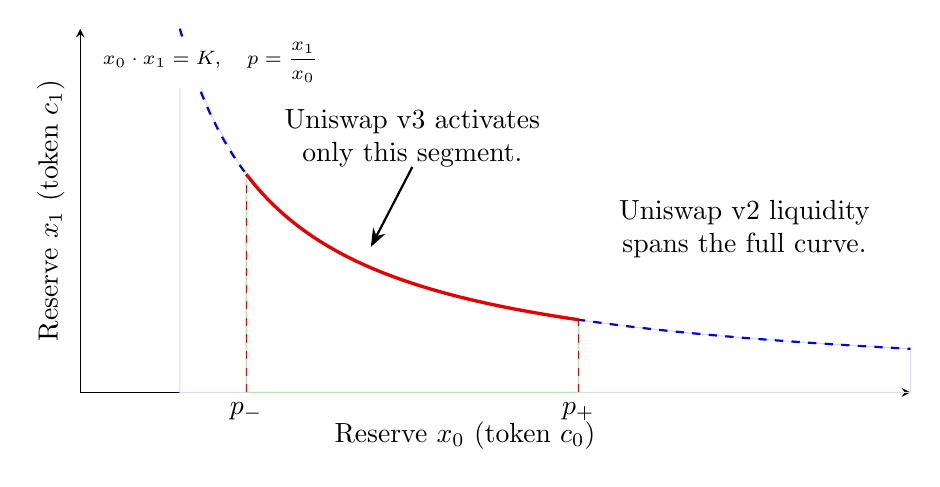
\begin{tikzpicture}[
  fill_v2/.style={blue!15, fill opacity=0.8},
  fill_v3/.style={green!30, fill opacity=0.8},
  plot_curve/.style={blue, thick},
  highlight_curve/.style={red, very thick},
]
\begin{axis}[
  xlabel={Reserve $x_0$ (token $c_0$)},
  ylabel={Reserve $x_1$ (token $c_1$)},
  axis lines=left,
  xmin=0, xmax=10,
  ymin=0, ymax=10,
  width=\linewidth, height=6.2cm,
  xtick=\empty, ytick=\empty,
  enlargelimits=false,
  clip=false,
  xlabel style={anchor=north, yshift=-5pt, xshift=-11pt},
  ylabel style={anchor=south},
]
% price band:
\def\pmin{2}
\def\pmax{6}

% v2 (full range)
\addplot [fill_v2, domain=1.2:10] {12/x} \closedcycle;

% v3 (concentrated range)
\addplot [fill_v3, domain=\pmin:\pmax] {12/x} \closedcycle;

% full bonding curve
\addplot [plot_curve, dashed, domain=1.2:10, samples=100] {12/x};

% active v3 segment
\addplot [highlight_curve, domain=\pmin:\pmax, samples=100] {12/x};

% price band markers
\draw[red, dashed] (axis cs:\pmin, 0) node[below=0.01pt, black] {\(p_{-}\)} -- (axis cs:\pmin, {12/\pmin});
\draw[red, dashed] (axis cs:\pmax, 0) node[below=0.01pt, black] {\(p_{+}\)} -- (axis cs:\pmax, {12/\pmax});

% labels (avoid “price” wording)
\node[text width=3.2cm, align=center] at (axis cs:8,4.5)
  {Uniswap v2 liquidity spans the full curve.};
\node[text width=3.5cm, align=center] at (axis cs:4,7)
  {Uniswap v3 activates only this segment.};
\draw[-Stealth, thick] (axis cs:4,6.2) -- (axis cs:3.5,4);

% small note: price definition
\node[anchor=north west, font=\scriptsize, fill=white, rounded corners=1pt, inner sep=2pt]
  at (rel axis cs:0.02,0.98) {$x_0 \cdot x_1=K,\quad p=\dfrac{x_1}{x_0}$};
\end{axis}
\end{tikzpicture}
\caption{Liquidity distribution in Uniswap v2 (full range) vs.\ Uniswap v3 (concentrated in \([p_{-},p_{+}]\)). The curve shows a constant-product contour \(x_0 \cdot x_1=K\), and the highlighted segment marks the price band where v3 liquidity is active.}
\label{fig:uniswap_fee_policy}
\end{figure}

\subsubsection{Fee microstructure and concentrated liquidity}
AMM protocols differ in how fees interact with liquidity.
In Uniswap v2, swap fees are \emph{reinvested into the pool reserves} on each trade, so the product $x_0 \cdot x_1{=}K$ grows.
In Uniswap v3, fees are added to the \emph{separate fee counters} of each position and do not change the active liquidity or the reserves until the LP explicitly claims or reinvests them.
Moreover, v3 allows LPs to choose a price band $[p_{-},p_{+}]$ and provide liquidity only inside it, as illustrated in Fig.~\ref{fig:uniswap_fee_policy}.
Let $p_{\text{pool}}$ denote the instantaneous pool price implied by reserves, defined as
$p_{\text{pool}} = x_1/x_0$. 
When $p_{\text{pool}}\in[p_{-},p_{+}]$, the position behaves locally like a Constant Product Market Maker (CPMM) with ``virtual'' reserves determined by $[p_{-},p_{+}]$ and its liquidity $L$, and it earns fees. 
If price exits this band, the position becomes out of range and is held entirely in a single asset, $c_0$ when $p_{\text{pool}}<p_{-}$ and $c_1$ when $p_{\text{pool}}>p_{+}$. 
In this out-of-range state, the position provides no active liquidity and therefore accrues no fees until the price re-enters the range or the LP rebalances.


\subsection{Impermanent Loss}
\label{sec:background_il}

\emph{Impermanent Loss} (IL) is the fundamental risk for liquidity providers in CFMMs. It is the relative underperformance of an LP's pool position versus a passive buy-and-hold (\emph{HODL}) strategy with the same initial assets~\cite{evans2021liquidity, aoyagi2020liquidity}.


\subsubsection{Mechanism and Formalization}
IL arises from the convex payout structure of the AMM invariant. When the relative market price of the pooled tokens changes, arbitrageurs trade against the pool to realign its internal price with external markets. This process forces the AMM to sell the appreciating asset and buy the depreciating asset, systematically reducing the total value of the pool relative to the HODL benchmark.
For a standard CPMM like Uniswap v2, where reserves $x_0, x_1$ satisfy $x_0 \cdot x_1 = K$, Tiruviluamala et al.~\cite{tiruviluamala2022general} derived the canonical closed-form expression for IL as a function of the price ratio change $R = p'/p$:
\begin{equation}
    \mathrm{IL}(R) = \frac{2\sqrt{R}}{1+R} - 1.
    \label{eq:il_canonical}
\end{equation}
This function is always non-positive ($\mathrm{IL} \le 0$) and symmetric with respect to log-returns, implying that LPs incur losses regardless of the direction of price divergence. While the loss is referred to as impermanent because it theoretically vanishes if prices return to their initial ratio (namely, $IL(R)=0$ for $R=1$), the path-dependent nature of volatility often crystallizes these losses upon withdrawal.

\subsubsection{Empirical Severity}
Empirical studies confirm that $IL \le 0$ is a pervasive feature of CFMM liquidity provision, while the ability of fees to offset it depends on pool type and market conditions. 
For Uniswap v2, stablecoin pairs tend to exhibit mild IL, whereas volatile or exotic pairs often experience IL that exceeds fee income~\cite{heimbach2021behavior, boueri2021g3m}. 
In Uniswap v3, concentrated liquidity can amplify divergence exposure, and passive narrow-range positions in volatile pools frequently realize net losses~\cite{heimbach2022risks}. 
Fee-aware analyses report that small price fluctuations can yield impermanent gain when fee flow is sufficiently strong, but this cushioning is limited under large divergence moves~\cite{roman2025impact}.


\subsection{Related Work}
Prior work studies LP risk in AMMs through IL theory and empirical evaluations across protocols. 
Canonical results derive closed-form IL for constant-product pools and extend it to broader CFMM families and multi-asset settings~\cite{tiruviluamala2022general}. 
Measured underperformance depends on the benchmark and on concentrated liquidity in Uniswap v3, where outcomes become range-dependent and can turn out-of-range~\cite{aigner2021uniswap, loesch2021impermanent, heimbach2022risks}. 
Related perspectives replace HODL with rebalancing-based references, such as LVR, and derive fee levels needed for fair compensation~\cite{milionis2022quantifying, milionis2022automated, cohen2023inefficiency}.
Recent work also shows that fee accounting can shift conclusions, and proposes fee-adjusted metrics such as RV and FARV for consistent evaluation across pools~\cite{roman2025impact, tangri2023generalizing}.



\section{Proxy-Based Statistical Metrics}
\label{sec:metrics}

{Section~\ref{sec:background_il} defines IL mechanically as a function of the realized relative price change over a holding period. In practice, this relative price change is uncertain at the time liquidity is provided, and its distribution varies across asset pairs and horizons. This motivates the statistical metrics introduced below, which summarize typical outcomes, downside risk, and the persistence of divergences using historical data.}

{In this paper, we interpret these metrics as \emph{ex-ante screening proxies}. Specifically, they are not intended to exactly value realized Uniswap v3 positions under concentrated liquidity. Instead, they provide a common full-range CPMM benchmark for comparing the inherent divergence risk of different token pairs before specifying a particular range-selection policy. This benchmark isolates pair-level relative-price risk and allows consistent cross-pool comparison without conflating it with strategy-specific choices such as band width, rebalancing, or out-of-range management. Later, in Section~\ref{sec:empirical_analysis}, we test whether the rankings induced by these proxy metrics remain informative when LP outcomes are evaluated under a higher-fidelity stylized Uniswap v3 simulation.}

{We employ three complementary proxy metrics that capture distinct aspects of divergence risk:}
\begin{enumerate}
    \item \textbf{{Mean-Variance Proxy:}} {Uses standard deviation to define typical risk boundaries under a common full-range benchmark.}
    \item \textbf{{Tail-Risk Proxy (5--95\%) Analysis:}} {Captures adverse divergence episodes using non-parametric quantiles.}
    \item \textbf{{Mean-Reversion Proxy:}} {Estimates the persistence of price-ratio shocks and serves as a horizon-management signal.}
\end{enumerate}

{Since these screening metrics are horizon-specific, we fix a holding horizon length $h$ (e.g., days, weeks, months) and define the corresponding $h$-period normalized price ratio by}
\(
    R^{(h)}_{t} \;=\; \frac{p_{t+h}}{p_t},
\)
{for each feasible start time $t$. Unless stated otherwise, we compute $\{R^{(h)}_{t}\}$ on a rolling basis, so consecutive ratios overlap in time rather than forming disjoint blocks. The proxy metrics below are computed from the empirical distribution $\mathcal{H}_{R^{(h)}}$ induced by the historical series $\{R^{(h)}_{t}\}$.}

\subsection{Mean and Standard Deviation Analysis}
{We start by characterizing the pool’s \emph{typical} divergence-risk environment under the common full-range benchmark. A traditional statistical approach to characterizing the distribution of the price ratio \(R^{(h)}\) involves its mean \(\mu_{R^{(h)}}\) and standard deviation (SD) \(\sigma_{R^{(h)}}\). These two moments are a cornerstone of classical statistical analysis and underpin many models in finance. Most notably, in Modern Portfolio Theory, they are used to define expected return and risk~\cite{markowitz1952portfolio, ross2014introduction}. Following this paradigm, we define the expected proxy IL based on the historical average of the \(h\)-period price ratio, \(\mu_{R^{(h)}}\), using the standard full-range CPMM formula:}
\begin{equation}
\label{eq:il_mean}
\mathrm{IL}_{\text{mean}} = \frac{2\sqrt{\mu_{R^{(h)}}}}{1+\mu_{R^{(h)}}} - 1.
\end{equation}

{We emphasize that $\mathrm{IL}_{\text{mean}}$ is used here as a screening statistic under a common benchmark, rather than as an exact estimate of realized Uniswap v3 payoff. The advantage of this construction is that it depends only on the historical relative-price path and therefore remains comparable across pools and fee tiers before one commits to a specific concentrated-liquidity policy.}

We note that as $\mathrm{IL}$ is nonlinear, in general
$\mathbb{E}[\mathrm{IL}(R^{(h)})] \neq \mathrm{IL}(\mathbb{E}[R^{(h)}])$.
{We adopt $\mathrm{IL}(\mu_{R^{(h)}})$ for $\mathrm{IL}_{\text{mean}}$ to maintain a mean--variance summary in the \emph{ratio} space. The mean $\mu_{R^{(h)}}$ captures the typical drift over horizon $h$, while dispersion and downside risk are quantified separately via $\sigma_{R^{(h)}}$ and the non-parametric tail metric introduced below.}

To establish a risk boundary that ensures validity (i.e., strictly positive price ratios), we adopt a log-normal approach. We compute the mean \(\mu_{Z}\) and standard deviation \(\sigma_{Z}\) of the log-ratios \(Z^{(h)} = \ln R^{(h)}\). The one-standard-deviation interval in log-space is \([\mu_{Z}-\sigma_{Z}, \mu_{Z}+\sigma_{Z}]\). Transforming this back to the price ratio space yields the interval \([\exp(\mu_{Z}-\sigma_{Z}), \exp(\mu_{Z}+\sigma_{Z})]\). We define the standard-deviation-based IL boundary, \(\mathrm{IL}_{\sigma\text{-bound}}\), by evaluating IL at the edges of this range:

\begin{equation}
\label{eq:il_sigma_bound}
\resizebox{\linewidth}{!}{$%
\mathrm{IL}_{\sigma\text{-bound}}
= \min\Biggl(
\frac{2\sqrt{\exp(\mu_{Z} - \sigma_{Z})}}{1+\exp(\mu_{Z} - \sigma_{Z})} - 1,\;
\frac{2\sqrt{\exp(\mu_{Z} + \sigma_{Z})}}{1+\exp(\mu_{Z} + \sigma_{Z})} - 1
\Biggr).
$}
\end{equation}

{This approach provides a compact proxy summary but is most informative when $\mathcal{H}_{R^{(h)}}$ is reasonably well-behaved. It is well documented that financial return distributions can exhibit skewness and heavy tails, which are not fully characterized by the mean and SD alone~\cite{mandelbrot2004fractals}. In such cases, the SD may underestimate the probability of extreme divergence events, motivating the use of non-parametric methods that are more robust to such distributional properties.}

\subsection{The 5--95 Percentile Metric}

{A mean--variance approach has several limitations, particularly its sensitivity to outliers and its implicit distributional assumptions. To address these issues, we employ a non-parametric 5--95 percentile proxy metric. We apply this metric to the empirical distribution of the $h$-period price ratio $R^{(h)}$. Let $\mathcal{H}_{R^{(h)}}$ denote the distribution induced by all historical observations $\{R^{(h)}_t\}$ for a given pool over the sample. The resulting percentiles are fixed summary statistics, meaning they are not indexed by time.}

We identify the 5th and 95th percentiles of this distribution, denoted $R^{(h)}_{0.05}$ and $R^{(h)}_{0.95}$, respectively.
{Using the same common full-range CPMM benchmark, we define the corresponding downside proxy, $\mathrm{IL}_{\text{bound}}$, as the more adverse (most negative) IL value at these percentile extremes:}
\begin{equation}
\label{eq:il_bound}
\mathrm{IL}_{\text{bound}} = \min\left(
\frac{2\sqrt{R^{(h)}_{0.05}}}{1+R^{(h)}_{0.05}} - 1,\quad
\frac{2\sqrt{R^{(h)}_{0.95}}}{1+R^{(h)}_{0.95}} - 1
\right).
\end{equation}

{This construction yields a downside screening threshold such that, in 90\% of observed $h$-period outcomes, the full-range proxy IL is not worse than $\mathrm{IL}_{\text{bound}}$. It therefore summarizes adverse relative-price divergence without requiring a commitment to a specific concentrated-liquidity range.}

Furthermore, we approximate the typical IL by using the median of \(\mathcal{H}_{R^{(h)}}\), denoted \(R^{(h)}_{\text{median}}\). The median-approximated IL is:
\begin{equation}
\label{eq:il_median}
\mathrm{IL}_{\text{median}} = \frac{2\sqrt{R^{(h)}_{\text{median}}}}{1+R^{(h)}_{\text{median}}} - 1.
\end{equation}

{To quantify sampling uncertainty in this non-parametric summary, we report a 95\% confidence interval for $\mathrm{IL}_{\text{median}}$ in the empirical section. This directly addresses the instability of point estimates in relatively short monthly samples and makes the screening layer more statistically transparent.}

\subsection{Mean-Reversion-Based Predictability Metric}
\label{subsubsec:mean_reversion_metric}

{Finally, we capture the persistence of relative-price shocks, i.e., how long divergence episodes tend to last. While the distributional proxy metrics above summarize the \emph{magnitude} of divergence risk, they do not describe the \emph{time dynamics} of the price ratio. For an LP, this distinction is crucial. When relative prices revert quickly after a shock, divergence-induced losses are more likely to remain temporary. When reversion is slow, divergence can persist for extended periods. To quantify this persistence, we evaluate how fast the price ratio returns toward a typical level after a deviation. Prior to estimating the AR(1) persistence metric, we perform an Augmented Dickey--Fuller (ADF) test as a basic stationarity diagnostic for the log price-ratio series.}

Let \(R_t\) denote the oriented price ratio sampled at the chosen frequency, and define the log-ratio \(Z_t = \ln R_t\).
We model \(Z_t\) with a basic mean-reverting model that describes how deviations from a long-run level \(\mu\) evolve over time:
\begin{equation}
\label{eq:ar1_ratio}
Z_{t+1} - \mu = \phi \bigl(Z_t - \mu\bigr) + \varepsilon_{t+1}, 
\qquad \varepsilon_{t+1} \stackrel{\mathrm{i.i.d.}}{\sim} N(0, \sigma^2_\varepsilon).
\end{equation}
Here, $0<\phi<1$ is a scalar that controls how quickly deviations die out, and \(\varepsilon_{t+1}\) is a random shock capturing new information in the market.
If \(|\phi|\) is close to 1, deviations shrink slowly and shocks can persist for many periods.
If \(|\phi|\) is smaller, deviations shrink faster and \(Z_t\) returns to \(\mu\) more quickly.

{We interpret this AR(1) specification as a reduced-form predictability proxy rather than a structural model of AMM dynamics. Its purpose is to summarize the persistence of pair-level relative-price shocks and thereby provide a simple horizon-management signal for the screening layer. In the empirical analysis, we supplement point estimates of $\hat{\phi}$ and $HL$ with uncertainty quantification and basic residual diagnostics.}

A convenient way to express the speed of reversion is the \emph{half-life} ($HL$), defined as the periods required for a deviation in $Z_t$ to decay by 50\%. For the AR(1) process $Z_t-\mu = \phi(Z_{t-1}-\mu)+\varepsilon_t$ with $0<\phi<1$, the half-life is:
\(
    HL = -\frac{\ln 2}{\ln \phi}.
\)
We exclude windows where $\hat{\phi} \notin (0,1)$ (e.g., near-unit-root cases), as $HL$ is then undefined. Shorter $HL$ implies higher predictability, as IL-inducing price deviations dissipate faster. Thus, $HL$ serves as a tool for horizon management, aligning LP lock-up periods with the expected speed of mean reversion.

\subsection{Tail-Adjusted Screening Metric (Net90)}
\label{subsec:net90}

The proxy metrics above summarize complementary aspects of pair-level divergence risk under the common full-range benchmark. In practice, however, pool screening also requires incorporating the fee side of liquidity provision. A pool with mild divergence risk may still be unattractive if fee generation is too weak, while a pool with stronger fee flow may remain viable despite moderate downside exposure. This motivates a simple tail-adjusted screening score that combines fee income with an adverse IL scenario.

Let $y^{\text{fee}}_t$ denote the realized fee yield over the chosen horizon and let $\mathrm{IL}_t$ denote the corresponding proxy IL realization under the common full-range benchmark. We define the \emph{Tail-Adjusted Yield} (\emph{Net90}) as
\begin{equation}
\label{eq:net90}
\mathrm{Net90}
=
\operatorname{median}\!\left(y^{\text{fee}}_{t}\right)
+
\operatorname{P}_{10}\!\left(\mathrm{IL}_{t}\right),
\end{equation}
where $\operatorname{P}_{10}(\mathrm{IL}_t)$ is the 10th percentile of the proxy-IL distribution across historical horizon-level observations.

Net90 is designed as an \emph{ex-ante screening score}. The first term captures the typical fee income available in the pool, while the second term imposes a downside adjustment based on a 90th-percentile adverse divergence event. Because $\mathrm{IL}_t \le 0$, the second term penalizes pools whose fee income is not sufficient to absorb large relative-price dislocations. Higher Net90 values therefore indicate pools whose structural fee generation remains more robust after accounting for tail divergence risk.

This metric should not be interpreted as an exact forecast of realized Uniswap v3 profitability under concentrated liquidity. Rather, like the other quantities in Section~\ref{sec:metrics}, it is a strategy-agnostic screening device under a common benchmark. Its role is to rank pools ex ante before specifying a particular concentrated-liquidity policy. In Section~\ref{sec:empirical_analysis}, we use Net90 as the main cross-pool screening score and then test whether the resulting ranking remains informative under stylized passive Uniswap v3 strategies.


\subsection{{Stylized Concentrated-Liquidity Valuation}}
\label{subsec:cl_valuation}

{The proxy metrics presented above summarize pair-level divergence risk under a common full-range CPMM benchmark. While this benchmark is useful for ex-ante screening and cross-pool comparison, actual Uniswap v3 positions are range-dependent and only earn fees while active within a chosen price interval. To connect the screening layer to realized passive LP outcomes, we introduce a stylized concentrated-liquidity valuation layer. This layer is used later in Section~\ref{sec:empirical_analysis} to simulate passive Uniswap v3 strategies under fixed price bands. It is not intended to model the full space of active LP management, but rather to provide a tractable validation setting for testing whether the proxy-based rankings remain informative under concentrated liquidity.}

{We consider a passive LP who enters a position at time $t_0$ when the pool price is $p_0$, chooses a fixed price range $[p_a,p_b]$, and holds the position until horizon end $t_1$ without rebalancing. In the empirical analysis, we study symmetric bands around the entry price, so that $p_a=(1-\delta)p_0$ and $p_b=(1+\delta)p_0$, where $\delta$ denotes the chosen concentration width. We evaluate several stylized widths, together with a full-range benchmark. We assume the LP provides liquidity passively, with no range updates, no fee compounding, and no transaction costs.}

{Let $L$ denote the liquidity parameter of the position. For a given terminal price $p_1$, the terminal inventory depends on whether the final price lies below, within, or above the selected range. Expressed in the numeraire of token~1, the terminal mark-to-market value of the position is given by the standard piecewise concentrated-liquidity formula}
\begin{equation}
\label{eq:v3_terminal_value}
V^{\mathrm{pos}}_1(p_1)=
\begin{cases}
L\left(\dfrac{1}{\sqrt{p_a}}-\dfrac{1}{\sqrt{p_b}}\right)p_1, & p_1 < p_a,\\[1.0em]
L\left(2\sqrt{p_1}-\sqrt{p_a}-\dfrac{p_1}{\sqrt{p_b}}\right), & p_a \le p_1 \le p_b,\\[1.0em]
L\left(\sqrt{p_b}-\sqrt{p_a}\right), & p_1 > p_b.
\end{cases}
\end{equation}

{This representation captures the defining feature of concentrated liquidity: When price exits the chosen band, the LP position is fully converted into a single asset and no longer behaves like an active two-sided liquidity position. As a consequence, both valuation and fee accrual become path-dependent.}

{To initialize the position, we normalize the LP’s entry wealth to a fixed notional $V_0$, identical across pools and strategy widths. Given the entry price $p_0$ and the chosen band $[p_a,p_b]$, this notional determines the implied liquidity $L$. This normalization ensures that realized outcomes are directly comparable across pools and concentration widths. As a benchmark, we compare the LP position against a passive HODL portfolio formed from the same initial token amounts at entry.}

{Unlike the ex-ante proxy metrics above, the concentrated-liquidity layer is evaluated on a daily path. For each day $t \in [t_0,t_1]$, we mark the LP position to market using the prevailing price $p_t$ and determine whether the position is active, i.e., whether $p_t \in [p_a,p_b]$. Fee income is accrued only on days when the position is in range. Because our dataset is pool-level rather than position-level, exact reconstruction of active-liquidity shares at each tick is not available. We therefore approximate daily fee income by allocating a fraction of the pool’s daily fees to the stylized LP conditional on the position being in range. This approximation should be interpreted as a reduced-form passive fee rule rather than an exact wallet-level accounting of realized Uniswap v3 fee claims.}

{Formally, let $y^{\mathrm{fee}}_t$ denote the daily fee income assigned to the stylized LP and let $\mathbf{1}\{p_t \in [p_a,p_b]\}$ be the indicator that the position is active on day $t$. The cumulative fee income over the holding horizon is then}
\begin{equation}
\label{eq:cum_fee_income}
Y^{\mathrm{fee}}_{t_0:t_1}
=
\sum_{t=t_0}^{t_1}
y^{\mathrm{fee}}_t \cdot \mathbf{1}\{p_t \in [p_a,p_b]\}.
\end{equation}

{Denoting the HODL terminal value by $V^{\mathrm{HODL}}_1(p_1)$, we define the realized passive concentrated-liquidity excess return over the episode as}
\begin{equation}
\label{eq:passive_v3_profit}
\Pi_{t_0:t_1}
=
\frac{V^{\mathrm{pos}}_1(p_1)+Y^{\mathrm{fee}}_{t_0:t_1}-V^{\mathrm{HODL}}_1(p_1)}{V_0}.
\end{equation}

{This quantity differs conceptually from the proxy metrics in Sections~III-A--III-C. The proxy layer is an ex-ante screening device based on pair-level divergence statistics under a common benchmark, whereas $\Pi_{t_0:t_1}$ is a realized passive-v3 outcome under a specific range choice. Comparing the ranking induced by the proxy layer to the ranking induced by $\Pi_{t_0:t_1}$ allows us to test when the simpler full-range metrics remain informative, and when concentrated liquidity materially alters the ordering across pools.}

{Finally, we emphasize the scope of this valuation layer. The proposed setup is deliberately stylized. It does not include active repositioning, dynamic range optimization, slippage, gas costs, or wallet-level fee reconstruction. Its purpose is narrower: to provide a controlled and transparent bridge between the paper’s proxy-based divergence-risk metrics and the realized behavior of passive concentrated-liquidity positions in Uniswap v3.}



\section{Empirical Analysis on Real Pools}
\label{sec:empirical_analysis}

{After presenting the proxy-based screening metrics in Section~\ref{sec:metrics}, we now apply them to real data from eight Uniswap v3 pools. The empirical analysis has two layers. First, we characterize and compare pools using the ex-ante screening proxies introduced in Section~\ref{sec:metrics}. Second, we evaluate whether the resulting rankings remain informative under a stylized passive Uniswap v3 simulation based on concentrated-liquidity valuation and daily path-dependent fee accrual.


\subsection{Data}

% \begin{table}[t]
% \centering
% \scriptsize
% \resizebox{0.5\textwidth}{!}{%
% \begin{tabular}{lll}
% \hline
% Pool address & Tokens & Fee tier\\
% \hline
% \texttt{0x4e68ccd3e89f51c3074ca5072bbac773960dfa36} & WETH/USDT & 0.30\% \\
% \texttt{0x11b815efb8f581194ae79006d24e0d814b7697f6} & WETH/USDT & 0.05\% \\
% \texttt{0x9db9e0e53058c89e5b94e29621a205198648425b} & WBTC/USDT & 0.30\% \\
% \texttt{0x4585fe77225b41b697c938b018e2ac67ac5a20c0} & WBTC/WETH & 0.05\% \\
% \texttt{0xcbcdf9626bc03e24f779434178a73a0b4bad62ed} & WBTC/WETH & 0.30\% \\
% \texttt{0x5ab53ee1d50eef2c1dd3d5402789cd27bb52c1bb} & AAVE/WETH & 0.30\% \\
% \texttt{0xa6cc3c2531fdaa6ae1a3ca84c2855806728693e8} & LINK/WETH & 0.30\% \\
% \texttt{0x1d42064fc4beb5f8aaf85f4617ae8b3b5b8bd801} & UNI/WETH & 0.30\% \\
% \hline
% \end{tabular}
% }
% \caption{Summary of Uniswap v3 pools used in the empirical analysis.}
% \label{tab:pools}
% \end{table}


\begin{table}[t]
\centering
\scriptsize
\resizebox{0.5\textwidth}{!}{%
\begin{tabular}{llll}
\hline
Pool ID & Tokens & Fee tier & Category\\
\hline
\texttt{4e} & WETH/USDT & 0.30\% & Stable--volatile\\
\texttt{11} & WETH/USDT & 0.05\% & Stable--volatile\\
\texttt{9d} & WBTC/USDT & 0.30\% & Stable--volatile\\
\texttt{45} & WBTC/WETH & 0.05\% & Volatile--volatile\\
\texttt{cb} & WBTC/WETH & 0.30\% & Volatile--volatile\\
\texttt{5a} & AAVE/WETH & 0.30\% & Governance-token\\
\texttt{a6} & LINK/WETH & 0.30\% & Governance-token\\
\texttt{1d} & UNI/WETH  & 0.30\% & Governance-token\\
\hline
\end{tabular}
}
\caption{Summary of Uniswap v3 pools used in the empirical analysis. }
\label{tab:pools}
\end{table}

We collect historical data for eight major Uniswap v3 liquidity pools using The Graph's public subgraph\footnote{https://thegraph.com/explorer}, covering 4.5 years (May~2021--December~2025). For each pool, we extract daily price, fee, and liquidity-related information and construct the normalized price-ratio series used in the proxy layer. The dataset covers two fee tiers (0.05\% and 0.30\%) and spans three pool categories: (i) stable--volatile pairs (WETH/USDT and WBTC/USDT), (ii) volatile--volatile pairs (WBTC/WETH), and (iii) governance-token pairs (AAVE/WETH, LINK/WETH, UNI/WETH), where AAVE, LINK, and UNI denote the Aave, Chainlink, and Uniswap tokens, respectively.
For reproducibility, we publish the raw data and scripts in an anonymous repository at \url{https://github.com/Profitable-Liquidity-Provision/paper-data}. 


The screening metrics in Section~\ref{sec:metrics} are intentionally computed using the standard full-range CPMM formula applied to observed price ratios. We use this as a common pair-level benchmark for divergence risk, enabling consistent comparisons across pools and fee tiers before specifying a particular concentrated-liquidity strategy. These quantities should therefore be interpreted as ex-ante screening proxies rather than exact valuations of realized Uniswap v3 positions.
At the same time, the empirical section goes beyond the proxy layer. In addition to the monthly screening analysis, we later evaluate stylized passive Uniswap v3 strategies using daily path-dependent simulation under fixed price bands. This second layer allows us to test whether pools favored by the simpler proxy metrics also perform well under concentrated liquidity.
During the analysis, we use the screening results at a one-month horizon. This interval matches a natural monitoring and repositioning frequency for LPs and yields enough observations over 4.5 years to estimate cross-pool risk summaries. By contrast, daily horizons are noisy and highly dependent, while annual horizons provide too few samples for stable estimation.




\begin{figure}[b]
    \centering
    % Monthly closing price p (series may be inverted in preprocessing if first close < 1)

\begin{tikzpicture}
  \begin{axis}[
    width=0.62\textwidth,
    height=0.35\textwidth,
    xlabel={Month},
    ylabel={Closing Price $p$},
    xmin=1, xmax=54,
    ymin=0,
    ymax=1.5*10^5,
    ymajorgrids=true,
    legend style={
      at={(1.2,0.96)},
      anchor=north west,
      font=\tiny,
      draw=black,
      fill=white,
      fill opacity=0.9,
      text opacity=1,
    },
    legend cell align={left},
    xmin=1, xmax=56,
    xtick={1,12,23,34,45,56},
    xticklabels={2021-05,2022-04,2023-03,2024-02,2025-01,2025-12},
    xticklabel style={font=\small},
    ymode=log,
  ]

    % -------------------------
    % WBTC/WETH (blue family, different markers)
    % -------------------------
    % 45: WBTC/WETH 0.05%
    \addplot+[
      color=blue!85!black,
      mark=x,
      line width=0.8pt
    ] table[
      col sep=comma,
      x expr=\coordindex+1,
      y=close
    ]{monthly_price/monthly_close_0x4585fe77225b41b697c938b018e2ac67ac5a20c0.csv};
    \addlegendentry{45: WBTC/WETH 0.05\%}

    % cb: WBTC/WETH 0.30%  (force it to be clearly blue + filled marker)
    \addplot+[
      color=blue!35!white,
      mark=pentagon*,
      mark options={fill=blue!35!white},
      line width=0.8pt
    ] table[
      col sep=comma,
      x expr=\coordindex+1,
      y=close
    ]{monthly_price/monthly_close_0xcbcdf9626bc03e24f779434178a73a0b4bad62ed.csv};
    \addlegendentry{cb: WBTC/WETH 0.30\%}

    % -------------------------
    % WETH/USDT (green family, different markers)
    % -------------------------
    % 4e: WETH/USDT 0.30%
    \addplot+[color=green!60!black, mark=*, mark options={fill=green!60!black}] table[
      col sep=comma,
      x expr=\coordindex+1,
      y=close
    ]{monthly_price/monthly_close_0x4e68ccd3e89f51c3074ca5072bbac773960dfa36.csv};
    \addlegendentry{4e: WETH/USDT 0.30\%}

    % 11: WETH/USDT 0.05%
    \addplot+[color=green!25!black, mark=diamond*, mark options={fill=green!25!black}] table[
      col sep=comma,
      x expr=\coordindex+1,
      y=close
    ]{monthly_price/monthly_close_0x11b815efb8f581194ae79006d24e0d814b7697f6.csv};
    \addlegendentry{11: WETH/USDT 0.05\%}

    % -------------------------
    % Distinct singletons
    % -------------------------
    % 9d: WBTC/USDT 0.30%
    \addplot+[color=violet!75!black, mark=triangle*, mark options={fill=violet!75!black}] table[
      col sep=comma,
      x expr=\coordindex+1,
      y=close
    ]{monthly_price/monthly_close_0x9db9e0e53058c89e5b94e29621a205198648425b.csv};
    \addlegendentry{9d: WBTC/USDT 0.30\%}

    % 5a: AAVE/WETH 0.30%  (moved away from red; clearly not blue)
    \addplot+[
      color=purple!75!black,
      mark=square*,
      mark options={fill=purple!75!black},
      dashed
    ] table[
      col sep=comma,
      x expr=\coordindex+1,
      y=close
    ]{monthly_price/monthly_close_0x5ab53ee1d50eef2c1dd3d5402789cd27bb52c1bb.csv};
    \addlegendentry{5a: AAVE/WETH 0.30\%}

    % a6: LINK/WETH 0.30%
    \addplot+[color=orange!85!black, mark=star, mark options={fill=orange!85!black}] table[
      col sep=comma,
      x expr=\coordindex+1,
      y=close
    ]{monthly_price/monthly_close_0xa6cc3c2531fdaa6ae1a3ca84c2855806728693e8.csv};
    \addlegendentry{a6: LINK/WETH 0.30\%}

    % 1d: UNI/WETH 0.30%
    \addplot+[color=cyan!80!black, mark=otimes*, mark options={fill=cyan!80!black}] table[
      col sep=comma,
      x expr=\coordindex+1,
      y=close
    ]{monthly_price/monthly_close_0x1d42064fc4beb5f8aaf85f4617ae8b3b5b8bd801.csv};
    \addlegendentry{1d: UNI/WETH 0.30\%}

  \end{axis}
\end{tikzpicture}

    \caption{Monthly closing price $p$ between May~2021 and December~2025.}
    \label{fig:monthly_pools_transformed}
\end{figure}

% \begin{figure}[t]
% \centering
% \resizebox{0.5\textwidth}{!}{%
%     \begin{tikzpicture}
  \begin{axis}[
    width=0.95\linewidth,
    height=0.7\linewidth,
    xlabel={Month},
    ylabel={Total Value Locked (USD)},
    xmin=1, xmax=56,
    ymode=log,
    ymin=1e5, ymax=1e9,
    ymajorgrids=true,
    xmajorgrids=false,
    xtick={1,13,25,37,49},
    xticklabels={2021-05,2022-05,2023-05,2024-05,2025-05},
    xticklabel style={
        font=\scriptsize,
        rotate=35,
        anchor=east
    },
    xlabel style={yshift=-0.5em},
    legend style={at={(0.02,0.02)},anchor=south west,font=\tiny,draw=black,fill=white,fill opacity=0.9,text opacity=1},
    legend cell align=left,
]

    % Data file: tvl_analysis/tvl_monthly_end.dat
    % Expected columns: month tvl_45 tvl_cb tvl_4e tvl_11 tvl_9d tvl_5a tvl_a6 tvl_1d

    % 45: WBTC/WETH 0.05%
    \addplot+[
      color=blue!85!black,
      mark=x,
      line width=0.8pt
    ] table[x=month,y=tvl_45] {tvl_analysis/tvl_monthly_end.dat};
    %\addlegendentry{45: WBTC/WETH 0.05\%}

    % cb: WBTC/WETH 0.30%
    \addplot+[
      color=blue!35!white,
      mark=pentagon*,
      mark options={fill=blue!35!white},
      line width=0.8pt
    ] table[x=month,y=tvl_cb] {tvl_analysis/tvl_monthly_end.dat};
    %\addlegendentry{cb: WBTC/WETH 0.30\%}

    % 4e: WETH/USDT 0.30%
    \addplot+[
      color=green!60!black,
      mark=*,
      mark options={fill=green!60!black},
      line width=0.8pt
    ] table[x=month,y=tvl_4e] {tvl_analysis/tvl_monthly_end.dat};
    %\addlegendentry{4e: WETH/USDT 0.30\%}

    % 11: WETH/USDT 0.05%
    \addplot+[
      color=green!25!black,
      mark=diamond*,
      mark options={fill=green!25!black},
      line width=0.8pt
    ] table[x=month,y=tvl_11] {tvl_analysis/tvl_monthly_end.dat};
    %\addlegendentry{11: WETH/USDT 0.05\%}

    % 9d: WBTC/USDT 0.30%
    \addplot+[
      color=violet!75!black,
      mark=triangle*,
      mark options={fill=violet!75!black},
      line width=0.8pt
    ] table[x=month,y=tvl_9d] {tvl_analysis/tvl_monthly_end.dat};
    %\addlegendentry{9d: WBTC/USDT 0.30\%}

    % 5a: AAVE/WETH 0.30%
    \addplot+[
      color=purple!75!black,
      mark=square*,
      mark options={fill=purple!75!black},
      dashed,
      line width=0.8pt
    ] table[x=month,y=tvl_5a] {tvl_analysis/tvl_monthly_end.dat};
    %\addlegendentry{5a: AAVE/WETH 0.30\%}

    % a6: LINK/WETH 0.30%
    \addplot+[
      color=orange!85!black,
      mark=star,
      mark options={fill=orange!85!black},
      line width=0.8pt
    ] table[x=month,y=tvl_a6] {tvl_analysis/tvl_monthly_end.dat};
    %\addlegendentry{a6: LINK/WETH 0.30\%}

    % 1d: UNI/WETH 0.30%
    \addplot+[
      color=cyan!80!black,
      mark=otimes*,
      mark options={fill=cyan!80!black},
      line width=0.8pt
    ] table[x=month,y=tvl_1d] {tvl_analysis/tvl_monthly_end.dat};
    %\addlegendentry{1d: UNI/WETH 0.30\%}

  \end{axis}
\end{tikzpicture}
% }
% \caption{Pool monthly total value locked (TVL), in USD.}
% \label{fig:monthly_tvl}
% \end{figure}

% \begin{figure}[t]
%     \centering
%     \resizebox{0.5\textwidth}{!}{%
%         \begin{tikzpicture}
  \begin{axis}[
    width=0.95\linewidth,
    height=0.72\linewidth,
    xlabel={Month},
    ylabel={Trading Volume (USD)},
    xmin=1, xmax=56,
    ymode=log,
    ymin=1e6, ymax=3e10,
    ymajorgrids=true,
    xmajorgrids=false,
    xtick={1,12,23,34,45,56},
    xticklabels={2021-05,2022-04,2023-03,2024-02,2025-01,2025-12},
    xticklabel style={
        font=\scriptsize,
        rotate=35,
        anchor=east
    },
    xlabel style={yshift=-0.5em},
    legend style={at={(0.02,0.02)},anchor=south west,font=\tiny,draw=black,fill=white,fill opacity=0.9,text opacity=1},
    legend cell align=left,
]

    % Data file: trading_volume/trading_volume_monthly.dat
    % Expected columns: month vol_45 vol_cb vol_4e vol_11 vol_9d vol_5a vol_a6 vol_1d

    % 45: WBTC/WETH 0.05%
    \addplot+[
      color=blue!85!black,
      mark=x,
      line width=0.8pt
    ] table[x=month,y=vol_45] {trading_volume/trading_volume_monthly.dat};
    %\addlegendentry{45: WBTC/WETH 0.05\%}

    % cb: WBTC/WETH 0.30%
    \addplot+[
      color=blue!35!white,
      mark=pentagon*,
      mark options={fill=blue!35!white},
      line width=0.8pt
    ] table[x=month,y=vol_cb] {trading_volume/trading_volume_monthly.dat};
    %\addlegendentry{cb: WBTC/WETH 0.30\%}

    % 4e: WETH/USDT 0.30%
    \addplot+[
      color=green!60!black,
      mark=*,
      mark options={fill=green!60!black},
      line width=0.8pt
    ] table[x=month,y=vol_4e] {trading_volume/trading_volume_monthly.dat};
    %\addlegendentry{4e: WETH/USDT 0.30\%}

    % 11: WETH/USDT 0.05%
    \addplot+[
      color=green!25!black,
      mark=diamond*,
      mark options={fill=green!25!black},
      line width=0.8pt
    ] table[x=month,y=vol_11] {trading_volume/trading_volume_monthly.dat};
    %\addlegendentry{11: WETH/USDT 0.05\%}

    % 9d: WBTC/USDT 0.30%
    \addplot+[
      color=violet!75!black,
      mark=triangle*,
      mark options={fill=violet!75!black},
      line width=0.8pt
    ] table[x=month,y=vol_9d] {trading_volume/trading_volume_monthly.dat};
    %\addlegendentry{9d: WBTC/USDT 0.30\%}

    % 5a: AAVE/WETH 0.30%
    \addplot+[
      color=purple!75!black,
      mark=square*,
      mark options={fill=purple!75!black},
      dashed,
      line width=0.8pt
    ] table[x=month,y=vol_5a] {trading_volume/trading_volume_monthly.dat};
    %\addlegendentry{5a: AAVE/WETH 0.30\%}

    % a6: LINK/WETH 0.30%
    \addplot+[
      color=orange!85!black,
      mark=star,
      mark options={fill=orange!85!black},
      line width=0.8pt
    ] table[x=month,y=vol_a6] {trading_volume/trading_volume_monthly.dat};
    %\addlegendentry{a6: LINK/WETH 0.30\%}

    % 1d: UNI/WETH 0.30%
    \addplot+[
      color=cyan!80!black,
      mark=otimes*,
      mark options={fill=cyan!80!black},
      line width=0.8pt
    ] table[x=month,y=vol_1d] {trading_volume/trading_volume_monthly.dat};
    %\addlegendentry{1d: UNI/WETH 0.30\%}

  \end{axis}
\end{tikzpicture}

%     }
%     \caption{Pool monthly total trading volume (in USD).}
%     \label{fig:monthly_pools_volume}
% \end{figure}

\begin{figure*}[t]
\centering

\begin{minipage}[t]{0.49\textwidth}
\centering
\resizebox{\textwidth}{!}{%
    \begin{tikzpicture}
  \begin{axis}[
    width=0.95\linewidth,
    height=0.7\linewidth,
    xlabel={Month},
    ylabel={Total Value Locked (USD)},
    xmin=1, xmax=56,
    ymode=log,
    ymin=1e5, ymax=1e9,
    ymajorgrids=true,
    xmajorgrids=false,
    xtick={1,13,25,37,49},
    xticklabels={2021-05,2022-05,2023-05,2024-05,2025-05},
    xticklabel style={
        font=\scriptsize,
        rotate=35,
        anchor=east
    },
    xlabel style={yshift=-0.5em},
    legend style={at={(0.02,0.02)},anchor=south west,font=\tiny,draw=black,fill=white,fill opacity=0.9,text opacity=1},
    legend cell align=left,
]

    % Data file: tvl_analysis/tvl_monthly_end.dat
    % Expected columns: month tvl_45 tvl_cb tvl_4e tvl_11 tvl_9d tvl_5a tvl_a6 tvl_1d

    % 45: WBTC/WETH 0.05%
    \addplot+[
      color=blue!85!black,
      mark=x,
      line width=0.8pt
    ] table[x=month,y=tvl_45] {tvl_analysis/tvl_monthly_end.dat};
    %\addlegendentry{45: WBTC/WETH 0.05\%}

    % cb: WBTC/WETH 0.30%
    \addplot+[
      color=blue!35!white,
      mark=pentagon*,
      mark options={fill=blue!35!white},
      line width=0.8pt
    ] table[x=month,y=tvl_cb] {tvl_analysis/tvl_monthly_end.dat};
    %\addlegendentry{cb: WBTC/WETH 0.30\%}

    % 4e: WETH/USDT 0.30%
    \addplot+[
      color=green!60!black,
      mark=*,
      mark options={fill=green!60!black},
      line width=0.8pt
    ] table[x=month,y=tvl_4e] {tvl_analysis/tvl_monthly_end.dat};
    %\addlegendentry{4e: WETH/USDT 0.30\%}

    % 11: WETH/USDT 0.05%
    \addplot+[
      color=green!25!black,
      mark=diamond*,
      mark options={fill=green!25!black},
      line width=0.8pt
    ] table[x=month,y=tvl_11] {tvl_analysis/tvl_monthly_end.dat};
    %\addlegendentry{11: WETH/USDT 0.05\%}

    % 9d: WBTC/USDT 0.30%
    \addplot+[
      color=violet!75!black,
      mark=triangle*,
      mark options={fill=violet!75!black},
      line width=0.8pt
    ] table[x=month,y=tvl_9d] {tvl_analysis/tvl_monthly_end.dat};
    %\addlegendentry{9d: WBTC/USDT 0.30\%}

    % 5a: AAVE/WETH 0.30%
    \addplot+[
      color=purple!75!black,
      mark=square*,
      mark options={fill=purple!75!black},
      dashed,
      line width=0.8pt
    ] table[x=month,y=tvl_5a] {tvl_analysis/tvl_monthly_end.dat};
    %\addlegendentry{5a: AAVE/WETH 0.30\%}

    % a6: LINK/WETH 0.30%
    \addplot+[
      color=orange!85!black,
      mark=star,
      mark options={fill=orange!85!black},
      line width=0.8pt
    ] table[x=month,y=tvl_a6] {tvl_analysis/tvl_monthly_end.dat};
    %\addlegendentry{a6: LINK/WETH 0.30\%}

    % 1d: UNI/WETH 0.30%
    \addplot+[
      color=cyan!80!black,
      mark=otimes*,
      mark options={fill=cyan!80!black},
      line width=0.8pt
    ] table[x=month,y=tvl_1d] {tvl_analysis/tvl_monthly_end.dat};
    %\addlegendentry{1d: UNI/WETH 0.30\%}

  \end{axis}
\end{tikzpicture}
}
\captionof{figure}{Pool monthly total value locked (TVL), in USD.}
\label{fig:monthly_tvl}
\end{minipage}
\hfill
\begin{minipage}[t]{0.49\textwidth}
\centering
\resizebox{\textwidth}{!}{%
    \begin{tikzpicture}
  \begin{axis}[
    width=0.95\linewidth,
    height=0.72\linewidth,
    xlabel={Month},
    ylabel={Trading Volume (USD)},
    xmin=1, xmax=56,
    ymode=log,
    ymin=1e6, ymax=3e10,
    ymajorgrids=true,
    xmajorgrids=false,
    xtick={1,12,23,34,45,56},
    xticklabels={2021-05,2022-04,2023-03,2024-02,2025-01,2025-12},
    xticklabel style={
        font=\scriptsize,
        rotate=35,
        anchor=east
    },
    xlabel style={yshift=-0.5em},
    legend style={at={(0.02,0.02)},anchor=south west,font=\tiny,draw=black,fill=white,fill opacity=0.9,text opacity=1},
    legend cell align=left,
]

    % Data file: trading_volume/trading_volume_monthly.dat
    % Expected columns: month vol_45 vol_cb vol_4e vol_11 vol_9d vol_5a vol_a6 vol_1d

    % 45: WBTC/WETH 0.05%
    \addplot+[
      color=blue!85!black,
      mark=x,
      line width=0.8pt
    ] table[x=month,y=vol_45] {trading_volume/trading_volume_monthly.dat};
    %\addlegendentry{45: WBTC/WETH 0.05\%}

    % cb: WBTC/WETH 0.30%
    \addplot+[
      color=blue!35!white,
      mark=pentagon*,
      mark options={fill=blue!35!white},
      line width=0.8pt
    ] table[x=month,y=vol_cb] {trading_volume/trading_volume_monthly.dat};
    %\addlegendentry{cb: WBTC/WETH 0.30\%}

    % 4e: WETH/USDT 0.30%
    \addplot+[
      color=green!60!black,
      mark=*,
      mark options={fill=green!60!black},
      line width=0.8pt
    ] table[x=month,y=vol_4e] {trading_volume/trading_volume_monthly.dat};
    %\addlegendentry{4e: WETH/USDT 0.30\%}

    % 11: WETH/USDT 0.05%
    \addplot+[
      color=green!25!black,
      mark=diamond*,
      mark options={fill=green!25!black},
      line width=0.8pt
    ] table[x=month,y=vol_11] {trading_volume/trading_volume_monthly.dat};
    %\addlegendentry{11: WETH/USDT 0.05\%}

    % 9d: WBTC/USDT 0.30%
    \addplot+[
      color=violet!75!black,
      mark=triangle*,
      mark options={fill=violet!75!black},
      line width=0.8pt
    ] table[x=month,y=vol_9d] {trading_volume/trading_volume_monthly.dat};
    %\addlegendentry{9d: WBTC/USDT 0.30\%}

    % 5a: AAVE/WETH 0.30%
    \addplot+[
      color=purple!75!black,
      mark=square*,
      mark options={fill=purple!75!black},
      dashed,
      line width=0.8pt
    ] table[x=month,y=vol_5a] {trading_volume/trading_volume_monthly.dat};
    %\addlegendentry{5a: AAVE/WETH 0.30\%}

    % a6: LINK/WETH 0.30%
    \addplot+[
      color=orange!85!black,
      mark=star,
      mark options={fill=orange!85!black},
      line width=0.8pt
    ] table[x=month,y=vol_a6] {trading_volume/trading_volume_monthly.dat};
    %\addlegendentry{a6: LINK/WETH 0.30\%}

    % 1d: UNI/WETH 0.30%
    \addplot+[
      color=cyan!80!black,
      mark=otimes*,
      mark options={fill=cyan!80!black},
      line width=0.8pt
    ] table[x=month,y=vol_1d] {trading_volume/trading_volume_monthly.dat};
    %\addlegendentry{1d: UNI/WETH 0.30\%}

  \end{axis}
\end{tikzpicture}

}
\captionof{figure}{Pool monthly total trading volume, in USD.}
\label{fig:monthly_pools_volume}
\end{minipage}

\end{figure*}

\subsection{General Pool Statistics}
\label{sec:general_statistics}

Fig.~\ref{fig:monthly_pools_transformed} presents the monthly closing price series $p$ for each analyzed Uniswap v3 pool. 
First, we note that the duplicated pairs (WETH--USDT and WBTC--USDT across two fee tiers) exhibit nearly identical prices in their respective pools. 
This holds even though each pool’s price is determined endogenously by its reserve ratio, rather than being set directly by the external market price.
This is because arbitrage traders trade against any deviation from the prevailing market price. Next, we observe the WETH--USDT pools (4e and 11) display a pronounced trough in mid-2022 (around June 2022), consistent with the sharp market drawdown in that period. By contrast, the WBTC--USDT pool (9d) evolves on a substantially larger scale and exhibits a different timing of its major decline (late 2022). Meanwhile, the cross-asset ratio pools (WBTC--WETH, AAVE--WETH, LINK--WETH, and UNI--WETH) remain on lower yet distinct levels with heterogeneous dynamics. 

Fig.~\ref{fig:monthly_tvl} presents the monthly total value locked (TVL) of the pools. 
Liquidity is highest in the WBTC/WETH 0.30\% pool (cb) and the WETH/USDT 0.30\% pool (4e), both of which persistently remain in the $10^{8}$ USD regime. 
Pool cb peaks at roughly $5\times10^{8}$ USD before retracing, while pool 4e trends upward and reaches about $3.6\times10^{8}$ USD near the end of the sample.
The corresponding lower-fee pools (45 for WBTC/WETH at 0.05\% and 11 for WETH/USDT at 0.05\%) begin with substantially smaller TVL but grow steadily over time. 
By late 2024, both pool 11 and the WBTC/USDT pool (9d) expand into the $\sim10^{8}$ USD range. 
Among the governance-token pools, LINK/WETH (a6) and UNI/WETH (1d) typically exhibit mid-range liquidity on the order of $10^{7}$--$10^{8}$ USD. 
In contrast, AAVE/WETH (5a) remains comparatively smaller, topping out at only a few $\times10^{7}$ USD.
We note all pools exhibit strictly positive daily TVL during every day in the sample, indicating continuous liquidity rather than intermittent data gaps.

% These TVL patterns show that liquidity differs widely across similar pools, so fee income likely depends on the liquidity regime, not just the fee tier.


Fig.~\ref{fig:monthly_pools_volume} presents the total monthly trading volume, measured in USD. 
Overall volume is dominated by the WETH/USDT pools (4e and 11) and the WBTC/WETH pools (45 and cb). 
Within this set, the low-fee WETH/USDT pool (11) exhibits the highest typical activity. 
Its monthly volume is frequently in the $10^{9}$--$10^{10}$ USD range and peaks above $5\times10^{9}$ USD. 
In contrast, the DeFi governance-token pools (AAVE/WETH, LINK/WETH, UNI/WETH) and the WBTC/USDT pool (9d) operate at materially lower volume levels on average.

Comparing pools with the \emph{same token pair} but different fee tiers reveals a clear trade-off between fee margin and capital velocity. 
Lower-fee pools often exhibit higher \emph{turnover} (monthly volume relative to TVL) due to order-flow routing, but higher activity does not automatically translate into higher returns. 
In particular, to outperform a 0.30\% fee tier, a 0.05\% pool must achieve turnover more than $6\times$ higher (since $0.30/0.05=6$) than its high-fee counterpart.

Our data illustrates that outcomes can differ across pairs. 
In May 2021, the WBTC/WETH 0.05\% pool (45) achieved turnover of $\approx57\times$, compared to $\approx5.4\times$ for the 0.30\% pool (cb). 
Because the turnover ratio ($\approx10.5\times$) exceeded the $6\times$ breakeven threshold, the lower-fee pool was the better choice. 
In contrast, for WETH/USDT in the same month, the 0.05\% pool (11) reached $\approx77\times$ turnover versus $\approx14\times$ for the 0.30\% pool (4e). 
Here the ratio ($\approx5.5\times$) fell short of the threshold, so the 0.30\% pool generated higher fee yield despite lower volume. 
This underscores that fee-tier comparisons should focus on \emph{fee velocity} ($\text{Fee Rate}\times\text{Turnover}$), rather than volume or fee rates alone.




\subsection{Proxy IL and Net-Loss Episodes}

The descriptive pool statistics above show that the pools differ substantially in price dynamics, liquidity, and trading activity. 
We next translate the observed monthly price-ratio movements into the full-range proxy IL benchmark introduced in Section~\ref{sec:metrics}. 
This allows us to compare divergence losses across pools before imposing any particular concentrated-liquidity range policy.

Fig.~\ref{fig:monthly_il} presents monthly full-range proxy IL computed from the observed monthly price ratio. These values should be interpreted as ex-post realizations of the common screening benchmark, not as exact valuations of concentrated-liquidity positions.
The two WETH/USDT pools (4e and 11) incurred the largest proxy IL losses during the mid--2022 drawdown. 
Their worst month was June~2022, with proxy IL of $\approx-3.91\%$ (4e) and $\approx-3.90\%$ (11).
In contrast, the correlated WBTC/WETH pools (45 and cb) experienced only mild proxy IL losses in June~2022 (about $-0.16\%$). 
However, both exhibited a regime change in mid--2025. 
Their maximum monthly proxy IL loss occurred in July~2025 at roughly $-1.33\%$, consistent with an idiosyncratic BTC--ETH divergence rather than a broad market shock.
The remaining pools fell into an intermediate risk band. 
WBTC/USDT (9d) and UNI/WETH (1d) showed larger proxy IL drawdowns in June~2022, at $\approx-2.56\%$ and $\approx-2.58\%$, respectively. 
LINK/WETH (a6) reached its worst month later, in May~2025, at about $-1.69\%$, while AAVE/WETH (5a) peaked in December~2024 at $\approx-3.24\%$.

\begin{figure}[t]
  \centering
        \begin{tikzpicture}
    \begin{axis}[
      width=0.32\textwidth,
      height=0.2\textheight,
      xmin=1,
      xmax=55,
      % --- UPDATED LIMITS (Scaled by 100) ---
      ymin=-4, 
      ymax=0.1, 
      xlabel={Month},
      ylabel={Monthly IL},
      xticklabel style={rotate=45, anchor=east, font=\tiny},
      xtick=\empty,
      extra x ticks={1,4,7,10,13,16,19,22,25,28,31,34,37,40,43,46,49,52,55},
      extra x tick style={xticklabel style={rotate=45, anchor=east, font=\tiny}},
      extra x tick labels={%
        2021-06,2021-09,2021-12,%
        2022-03,2022-06,2022-09,2022-12,%
        2023-03,2023-06,2023-09,2023-12,%
        2024-03,2024-06,2024-09,2024-12,%
        2025-03,2025-06,2025-09,2025-12},
      scaled y ticks=false,
      % --- DATA FILTER (Multiplies y-values by 100) ---
      y filter/.code={\pgfmathparse{\pgfmathresult*100}\pgfmathresult},
      % --- UPDATED TICKS & LABELS ---
      yticklabel style={/pgf/number format:fixed, /pgf/number format:precision=1},
      yticklabel={\pgfmathprintnumber{\tick}\%}, % Adds the % sign
      ytick={-4,-3.5,-3,-2.5,-2,-1.5,-1,-0.5,0},
      grid=both,
      legend style={
        at={(1.31,0.02)},
        anchor=south,
        legend columns=1,
        font=\tiny,
        draw=black,
        fill=white,
        fill opacity=0.9,
        text opacity=1,
      },
      legend cell align=left,
    ]

      % Data file: monthly_il/monthly_il.dat
      % 45: WBTC/WETH 0.05%
      \addplot+[
        color=blue!85!black,
        mark=x,
        mark size=1.2pt,
        line width=0.8pt
      ] table[x=month,y=il_45] {monthly_il/monthly_il.dat};
      \addlegendentry{45: WBTC/WETH 0.05\%}

      % cb: WBTC/WETH 0.30%
      \addplot+[
        color=blue!35!white,
        mark=pentagon*,
        mark options={fill=blue!35!white},
        mark size=1.2pt,
        line width=0.8pt
      ] table[x=month,y=il_cb] {monthly_il/monthly_il.dat};
      \addlegendentry{cb: WBTC/WETH 0.30\%}

      % 4e: WETH/USDT 0.30%
      \addplot+[
        color=green!60!black,
        mark=*,
        mark options={fill=green!60!black},
        mark size=1.2pt,
        line width=0.8pt
      ] table[x=month,y=il_4e] {monthly_il/monthly_il.dat};
      \addlegendentry{4e: WETH/USDT 0.30\%}

      % 11: WETH/USDT 0.05%
      \addplot+[
        color=green!25!black,
        mark=diamond*,
        mark options={fill=green!25!black},
        mark size=1.2pt,
        line width=0.8pt
      ] table[x=month,y=il_11] {monthly_il/monthly_il.dat};
      \addlegendentry{11: WETH/USDT 0.05\%}

      % 9d: WBTC/USDT 0.30%
      \addplot+[
        color=violet!75!black,
        mark=triangle*,
        mark options={fill=violet!75!black},
        mark size=1.2pt,
        line width=0.8pt
      ] table[x=month,y=il_9d] {monthly_il/monthly_il.dat};
      \addlegendentry{9d: WBTC/USDT 0.30\%}

      % 5a: AAVE/WETH 0.30%
      \addplot+[
        color=purple!75!black,
        mark=square*,
        mark options={fill=purple!75!black},
        dashed,
        mark size=1.2pt,
        line width=0.8pt
      ] table[x=month,y=il_5a] {monthly_il/monthly_il.dat};
      \addlegendentry{5a: AAVE/WETH 0.30\%}

      % a6: LINK/WETH 0.30%
      \addplot+[
        color=orange!85!black,
        mark=star,
        mark options={fill=orange!85!black},
        mark size=1.6pt,
        line width=0.8pt
      ] table[x=month,y=il_a6] {monthly_il/monthly_il.dat};
      \addlegendentry{a6: LINK/WETH 0.30\%}

      % 1d: UNI/WETH 0.30%
      \addplot+[
        color=cyan!80!black,
        mark=otimes*,
        mark options={fill=cyan!80!black},
        mark size=1.2pt,
        line width=0.8pt
      ] table[x=month,y=il_1d] {monthly_il/monthly_il.dat};
      \addlegendentry{1d: UNI/WETH 0.30\%}

      % zero line for reference
      % Note: 0 scaled by 100 is still 0
      \addplot[black, thick] coordinates {(1,0) (55,0)};

    \end{axis}
\end{tikzpicture}
  \caption{Monthly full-range proxy IL.}
  \label{fig:monthly_il}
\end{figure}

Under this hybrid screening benchmark, which combines observed pool fee yield with full-range proxy divergence loss, all eight pools exhibit months in which fee yield is insufficient to offset the proxy IL loss, as summarized in Table~\ref{tab:worst_net_loss}. These hybrid proxy net-loss episodes show that divergence risk is economically meaningful even before concentrated-liquidity effects are introduced. They therefore motivate the screening layer and provide a baseline against which the stylized passive Uniswap v3 results can later be compared.

\begin{table}[b]
\centering
\footnotesize
\begin{tabular}{lccccc}
\toprule
Pool & Fee tier & Month & Fee yield & Proxy IL & Hybrid net \\
\midrule
45 & 0.05\% & Jul 25 & 0.13\% & -1.33\% & -1.21\% \\
cb & 0.30\% & Jul 25 & 0.08\% & -1.34\% & -1.25\% \\
4e & 0.30\% & Feb 24 & 0.56\% & -1.88\% & -1.32\% \\
11 & 0.05\% & Jul 25 & 0.98\% & -2.19\% & -1.20\% \\
9d & 0.30\% & Jan 23 & 0.65\% & -1.26\% & -0.62\% \\
5a & 0.30\% & Jul 25 & 1.28\% & -2.24\% & -0.97\% \\
a6 & 0.30\% & May 25 & 0.50\% & -1.69\% & -1.18\% \\
1d & 0.30\% & Jun 22 & 1.28\% & -2.58\% & -1.30\% \\
\bottomrule
\end{tabular}
\caption{Proxy net-loss examples under the full-range screening benchmark.}
\label{tab:worst_net_loss}
\end{table}

\subsection{Cross-Pool Proxy IL Risk Metrics}

After documenting individual proxy IL episodes, we next compare the pools through the distributional screening metrics. 
We now move from isolated monthly loss episodes to cross-pool risk summaries that can be used ex ante. 
We begin with the monthly price-ratio distribution, which is the object that drives proxy IL over the LP holding horizon.


Fig.~\ref{fig:mean_std_R} presents the empirical mean and SD of the monthly price ratio for each pool.
Unlike Fig.~\ref{fig:monthly_pools_transformed}, this construction aligns with a one-month LP holding horizon by measuring within-month relative price movements.
Across pools, the mean ratios remain close to unity (approximately \(0.987\)--\(1.039\)), implying that typical monthly drift in the relative price is small compared to its dispersion.
The dispersion, however, varies substantially. The WETH/USDT pools (4e, 11) exhibit the largest month-to-month variability
(\(\sigma \approx 0.218\)--\(0.219\)), whereas the correlated WBTC/WETH pools (45, cb) are much more stable
(\(\sigma \approx 0.120\)).
The remaining pools fall in an intermediate band, with WBTC/USDT (9d) around \(\sigma \approx 0.161\) and the DeFi token pairs AAVE/WETH, LINK/WETH, and UNI/WETH (5a, a6, 1d) around \(\sigma \approx 0.168\)--\(0.173\).
This demonstrates how cross-pool differences at the one-month horizon are driven mainly by dispersion rather than drift. 
As a result, stable--volatile pairs exhibit higher typical proxy IL exposure than correlated volatile--volatile pairs.

\begin{figure*}[t]
\centering

\begin{minipage}[t]{0.35\textwidth}
\centering
\resizebox{\textwidth}{!}{%
        \begin{tikzpicture}
        \begin{axis}[
            ybar,
            width=1.6\textwidth,
            height=0.84\textwidth,
            ylabel={Mean / SD},
            symbolic x coords={45,cb,4e,11,9d,5a,a6,1d},
            xtick=data,
            x tick label style={rotate=45,anchor=east},
            legend style={at={(0.02,0.82)},anchor=north west, font=\small},
            bar width=9pt,
            enlarge x limits=0.08,
            ymajorgrids=true,
            %ymode=log,
            grid style={dotted},
            % make y-axis easier to read
            ymin=0, ymax=1.1,
            ytick={0, 0.2,0.4,0.6,0.8,1},
            yticklabel style={/pgf/number format:fixed,/pgf/number format:precision=2},
        ]

        % Mean(R^{(1m)})
        \addplot table[
            col sep=tab,
            x=pool_short,
            y=mean_R_month
        ] {monthly_R/monthly_R_stats_summary.dat};
        \addlegendentry{Mean of $R^{(1m)}_t$}

        % Std(R^{(1m)})
        \addplot table[
            col sep=tab,
            x=pool_short,
            y=std_R_month
        ] {monthly_R/monthly_R_stats_summary.dat};
        \addlegendentry{SD\ of $R^{(1m)}_t$}

        \end{axis}
    \end{tikzpicture}
}
\captionof{figure}{Monthly price ratio mean and SD.}
\label{fig:mean_std_R}
\end{minipage}
\hfill
\begin{minipage}[t]{0.64\textwidth}
\centering
\resizebox{\textwidth}{!}{%
    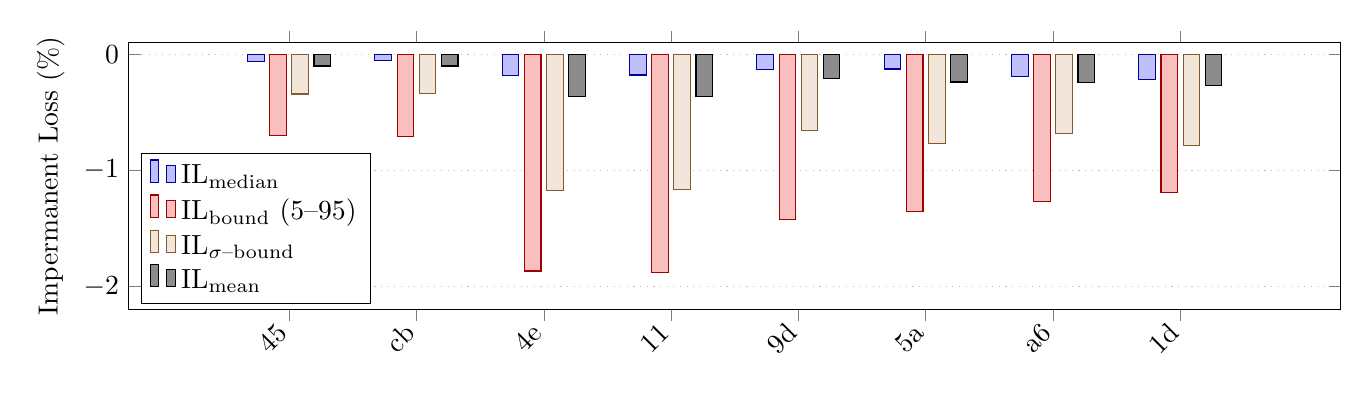
\begin{tikzpicture}
\begin{axis}[
    width=1.4\textwidth,
    height=0.41\textwidth,
    ybar,
    bar width=6pt,
    enlarge x limits=0.18,
    ymin=-2.2, ymax=0.1,
    ymajorgrids=true,
    grid style={dotted},
    ylabel={Impermanent Loss (\%)},
    symbolic x coords={45,cb,4e,11,9d,5a,a6,1d},
    xtick=data,
    xticklabel style={rotate=45, anchor=east},
    legend style={
        at={(0.01,0.02)},
        anchor=south west,
        draw=black,
        fill=white,
        %font=\Large,
    },
    legend cell align={left},
]

% IL_median
\addplot[draw=blue!70!black, fill=blue!25, bar shift=-12pt] coordinates { (45,-0.062025) (cb,-0.053979) (4e,-0.184368) (11,-0.179866) (9d,-0.133229) (5a,-0.127624) (a6,-0.191402) (1d,-0.217280) };
\addlegendentry{$\mathrm{IL}_{\text{median}}$}

% IL_bound (5--95)
\addplot[draw=red!70!black, fill=red!25, bar shift=-4pt] coordinates { (45,-0.698558) (cb,-0.708234) (4e,-1.867968) (11,-1.879260) (9d,-1.420822) (5a,-1.353484) (a6,-1.269196) (1d,-1.191524) };
\addlegendentry{$\mathrm{IL}_{\text{bound}}~(5\text{--}95)$}

% IL_sigma-bound
\addplot[draw=brown!70!black, fill=brown!20, bar shift=4pt] coordinates { (45,-0.343281) (cb,-0.342155) (4e,-1.173647) (11,-1.166907) (9d,-0.655256) (5a,-0.770508) (a6,-0.683694) (1d,-0.786992) };
\addlegendentry{$\mathrm{IL}_{\sigma\text{--}\text{bound}}$}

% IL_mean
\addplot[draw=black, fill=black!45, bar shift=12pt] coordinates { (45,-0.102314) (cb,-0.102141) (4e,-0.367057) (11,-0.366243) (9d,-0.207247) (5a,-0.240038) (a6,-0.242804) (1d,-0.272718) };
\addlegendentry{$\mathrm{IL}_{\text{mean}}$}

\end{axis}
\end{tikzpicture}

}
\captionof{figure}{Monthly proxy IL screening-metric summary.}
\label{fig:monthly_il_summary_metrics}
\end{minipage}

\end{figure*}

We next summarize the monthly full-range proxy IL distribution using the four screening metrics from Section~\ref{sec:metrics}. Fig.~\ref{fig:monthly_il_summary_metrics} reports $\mathrm{IL}_{\text{median}}$, $\mathrm{IL}_{\text{bound}}~(5\text{--}95)$, $\mathrm{IL}_{\sigma\text{-bound}}$, and $\mathrm{IL}_{\text{mean}}$. These statistics provide an ex-ante screening view of pair-level divergence risk under the common full-range benchmark.
First, in this sample, the metrics consistently separated the pools into clear proxy-risk tiers. The WBTC/WETH pools (45 and cb) exhibited the smallest proxy IL losses across all summaries. Their typical monthly proxy IL was close to zero (medians $\approx-0.062\%$ and $\approx-0.054\%$) and their proxy downside exposure was markedly milder than the rest (5--95 bounds around $-0.70\%$). At the opposite end, the WETH/USDT pools (4e and 11) displayed the largest systematic proxy IL, with the most negative means (both $\approx$ $-0.367\%$) and the deepest proxy downside bounds (5--95 bounds near $-1.87\%$ and $\sigma$-bounds around $-1.17\%$). 
The remaining pools formed an intermediate proxy-risk regime, having medians between roughly $-0.13\%$ and $-0.22\%$. Meanwhile, their proxy downside bounds were substantially less severe than the WETH/USDT group (5--95 bounds between $\approx$ $-1.19\%$ and $-1.42\%$). This indicated meaningfully smaller proxy tail exposure despite non-negligible typical proxy IL.

The second trend was that the four screening metrics emphasized different aspects of proxy IL risk. 
As a result, they could alter the relative ranking within the intermediate tier. 
For example, 1d had the most negative median among the intermediate pools ($\approx-0.217\%$), indicating weaker median-month proxy performance. 
However, its downside bound was the shallowest in that tier (5--95 bound $\approx-1.19\%$), implying comparatively stronger proxy tail protection. 
Conversely, 9d had a less negative median ($\approx-0.133\%$) but a deeper 5--95 bound ($\approx-1.42\%$), reflecting more severe adverse-month proxy exposure. 
Similarly, a6 and 5a had comparable means ($\approx-0.243\%$ and $-0.240\%$) but differed in proxy tail behavior (5--95 bounds $\approx-1.27\%$ versus $\approx-1.35\%$). 
This illustrated that pools could share similar average proxy IL while differing in the severity of rare dislocations.


\begin{figure}[t]
\centering
\resizebox{0.5\textwidth}{!}{%
        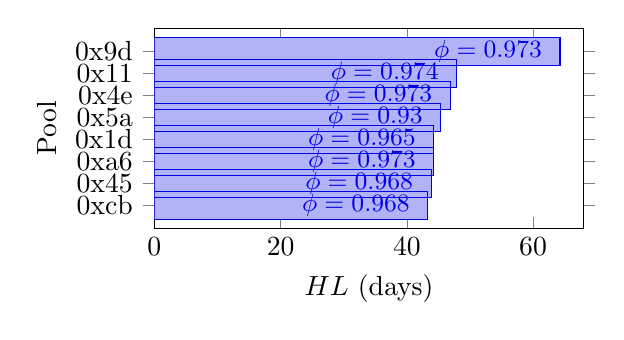
\begin{tikzpicture}
  \begin{axis}[
    xbar,
    width=0.58\textwidth,
    height=0.34\textwidth,
    xlabel={$HL$ (days)},
    ylabel={Pool},
    % order bars by HalfLife (largest at top), matching the new results:
    symbolic y coords={0x9d,0x11,0x4e,0x5a,0x1d,0xa6,0x45,0xcb},
    ytick=data,
    y dir=reverse,
    xmin=0,
    xmax=68,
    bar width=10pt,
    enlarge y limits=0.15,
    point meta=explicit,
    nodes near coords={$\phi=\pgfmathprintnumber[fixed,precision=3]{\pgfplotspointmeta}$},
    nodes near coords style={
        anchor=east,
        xshift=-3pt,
        font=\small
    },
  ]

    % (half-life, pool-id) [mean phi]
    \addplot coordinates {
      (64.26,0x9d) [0.973] % 9d  WBTC/USDT
      (47.89,0x11) [0.974] % 11  WETH/USDT 0.05%
      (46.88,0x4e) [0.973] % 4e  WETH/USDT 0.30%
      (45.39,0x5a) [0.930] % 5a  AAVE/WETH 0.30%
      (44.28,0x1d) [0.965] % 1d  UNI/WETH 0.30%
      (44.28,0xa6) [0.973] % a6  LINK/WETH 0.30%
      (43.84,0x45) [0.968] % 45  WBTC/WETH 0.05%
      (43.33,0xcb) [0.968] % cb  WBTC/WETH 0.30%
    };

  \end{axis}
\end{tikzpicture}

    }
\caption{Mean 180-day rolling $HL$, with the corresponding mean AR(1) coefficient $\phi$.}
\label{fig:half_life_180d_mean_phi_inside}
\end{figure}

Fig.~\ref{fig:half_life_180d_mean_phi_inside} presents the mean 180-day rolling $HL$ and AR(1) coefficient $\phi$, computed from overlapping 180-day windows. 
For each pool, we construct an adjusted price series $P_{\text{adj},t}$ (inverted when its mean is below unity) and fit an AR(1) model to the log prices, $Z_t=\ln P_{\text{adj},t}$. 
The window-specific coefficients $\phi_t$ are converted to half-lives via $\mathrm{HL}_t=-\ln 2 / \ln \phi_t$.
Prior to estimating persistence, we perform an Augmented Dickey--Fuller (ADF) test as a basic stationarity diagnostic for the log price-ratio series. 
The resulting half-lives provide reduced-form summaries of relative-price persistence, not structural estimates of AMM dynamics.
The figure shows that price deviations in these markets were persistent, but persistence differed materially across pools. 
The mean $HL$ ranged from $43.33$ to $64.26$ days, while the mean AR(1) coefficients spanned approximately $0.930$ to $0.974$, implying that price-ratio shocks typically decayed over several weeks to roughly two months. 
Because the mapping from $\phi$ to $HL$ is highly nonlinear as $\phi\to 1$, small differences in persistence could translate into meaningful differences in expected shock duration.
This effect was evident in the top-ranked pool 9d (WBTC/USDT), which attained the longest mean $HL$ ($64.26$ days) despite having $\phi\approx0.973$, similar to pools 4e and 11. 
This suggests that near-unit-root episodes in some windows disproportionately increased average $HL$, even when mean $\phi$ values were similar.

Additionally, analyzing the results by pool type revealed a revised cross-sectional pattern.
The WBTC/USDT pool 9d was the most persistent market by a wide margin. 
This implies that deviations between BTC and the dollar-pegged asset could remain sticky for extended periods, potentially sustaining proxy IL exposure over longer horizons.
In contrast, the two WBTC/WETH pools (45, cb) sat at the bottom of the ranking (mean $HL\approx 43$--$44$ days), consistent with faster relative adjustment between two major crypto-assets. 
The WETH/USDT pools (11, 4e) formed an intermediate cluster around $\approx 47$ days, indicating persistence that was substantial but below the BTC--stablecoin case. 
Beyond the stablecoin-based pools, the  governance token pairs occupied a broader middle band.
Pool 5a (AAVE/WETH) exhibited the lowest mean $\phi$ ($\approx0.930$) yet still had $HL\approx45$ days. 
Pools 1d (UNI/WETH) and a6 (LINK/WETH) were close in $HL$ (both $\approx44.28$ days) despite differing mean $\phi$ values. 
This underscored that average $HL$ could be shaped by the distribution of window-level persistence, not the mean coefficient alone.
Overall, none of the pools exhibited rapid mean reversion. Instead, pair-level shocks tended to decay gradually over the medium term, implying that divergence episodes can remain relevant over realistic LP holding horizons.


\subsection{Recursive Calibration of Proxy IL Metrics}
\label{subsec:backtesting_il}

The IL analysis above provides an \emph{ex post} summary of historical risk under the full-range proxy benchmark. 
To test whether the historical proxy summaries remain informative for subsequent months under the same full-range benchmark, we run a recursive calibration exercise.
For each pool and month $t$ (starting at $t=13$), we estimated the four presented metrics: $\mathrm{IL}_{\text{bound}}$, $\mathrm{IL}_{\sigma\text{-bound}}$, $\mathrm{IL}_{\text{median}}$, and $\mathrm{IL}_{\text{mean}}$. We use an expanding window that included only data prior to month $t$. 
This produced an \emph{ex ante} historical-risk estimate, denoted $\mathrm{IL}^{(t)}_{\text{estimate}}$, which we compare with the realized proxy IL in month $t$, denoted $\mathrm{IL}^{(t)}_{\text{real}}$.
We then computed the exceedance rate $\hat{\alpha}$, the fraction of out-of-sample months where realized proxy IL was worse (more negative) than the historical-risk estimate:
\(
\hat{\alpha}
= \frac{1}{T_{\text{oos}}}\sum_{t=1}^{T_{\text{oos}}}
\mathbf{1}\!\left\{\mathrm{IL}^{(t)}_{\text{real}} < \mathrm{IL}^{(t)}_{\text{estimate}}\right\},
\)
where $T_{\text{oos}}$ is the number of out-of-sample months. 
For a stable distribution, the nonparametric 10\% lower-tail bound should have an exceedance rate near $0.10$. The normal-reference $\sigma$-bound has a one-sided benchmark of approximately $0.16$ under the normal approximation for $\ln R^{(h)}$. The median has a natural exceedance benchmark of $0.50$. The mean does not define a quantile target for a skewed IL distribution, so its exceedance rate is reported descriptively rather than treated as a formal calibration target.

Fig.~\ref{fig:backtest_scores_heatmap} visualized these exceedance rates after converting them into normalized calibration scores to facilitate cross-metric comparison. 
For each metric, we mapped $\hat{\alpha}$ to a unit-scale score in $[0,1]$ based on its deviation from the target exceedance level $\alpha^\star$. 
Under this normalization, a score of $1$ indicated perfect calibration, and lower scores indicated larger deviations from the target.
For the mean metric, the score is included only as a descriptive comparison using $0.50$ as a symmetry benchmark, not as a formal calibration target.
The results show distinct heterogeneity in performance across pools. 
For some pools (e.g., 9d), the 10\% bound ($\mathrm{IL}_{\text{bound}}$) was well-calibrated, yielding $\hat{\alpha}\approx0.093$, close to the theoretical target of $0.10$. 
Conversely, pools such as 45 and cb exhibited higher exceedance rates ($\hat{\alpha}\approx0.186$), indicating that historical proxy summaries tended to underestimate subsequent full-range downside risk. 
Moreover, for most pools, the median exceedance rate fell below $0.50$ (roughly $0.33$--$0.35$), suggesting conservative historical-risk estimates for typical months but weaker coverage of extreme downside events.
This implies that calibration quality is pool-dependent and that tail-oriented proxy metrics can under-cover future full-range proxy IL in the presence of heavy-tailed divergence shocks.

\begin{figure}[b]
    \centering
\includegraphics[width=0.53\textwidth]{backtesting_analysis.tex}
\caption{Normalized recursive-calibration scores for proxy IL metrics.}
\label{fig:backtest_scores_heatmap}
\end{figure}

\subsection{Stylized Passive Uniswap v3 Simulation and Proxy Alignment}
\label{subsec:stylized_v3_validation}

The recursive calibration analysis above evaluates the historical-risk estimates under the common full-range proxy benchmark. 
While this is useful for assessing the internal consistency of the screening layer, it does not by itself show how the proxy metrics behave once protocol-specific LP mechanics are introduced. 
We therefore complement the proxy analysis with a stylized passive Uniswap v3 simulation, using Uniswap v3 as a demanding empirical setting because concentrated liquidity makes outcomes range-dependent. 
LP positions are simulated under fixed price bands and evaluated using daily path-dependent valuation and fee accrual. 
This allows us to examine whether proxy-based pool rankings remain aligned with realized passive outcomes after concentrated-liquidity mechanics are introduced explicitly.

\subsubsection{Stylized passive-v3 simulation by pool and band}

We begin by simulating stylized passive Uniswap v3 positions for each pool under a small menu of fixed range policies. For each monthly episode, an LP enters at the start-of-month price and holds the position passively until month-end, without rebalancing. We consider a full-range benchmark together with three symmetric concentrated-liquidity bands around the entry price, namely $\pm20\%$, $\pm10\%$, and $\pm5\%$. The bands $\pm20\%$, $\pm10\%$, and $\pm5\%$ are not optimized strategies. They are simple passive range policies chosen to span wide, moderate, and tight concentration regimes. The full-range strategy serves as the broad-exposure benchmark within the same stylized Uniswap v3 simulation framework.

For each pool-month and each range policy, the LP enters at the start-of-month price with normalized initial capital. The token amounts and liquidity are computed using the Uniswap v3 valuation formulas for the chosen price range. Each day, the position is revalued using the observed pool price. Fees accrue only when the price is inside the selected range and are allocated according to the position's active liquidity relative to pool liquidity. Fees are accumulated separately and are not reinvested. The monthly excess return is the final LP value, including accrued fees, minus the value of a HODL portfolio initialized with the same start-of-month token amounts. Gas costs, slippage, and active repositioning are excluded.



\begin{table*}[t]
\centering
\scriptsize
\setlength{\tabcolsep}{5pt}
\begin{tabular}{llrrr}
\toprule
Pool & Strategy & Median excess return (\%) & 10th pct. excess return (\%) & Active share (\%) \\
\midrule
4e & full\_range & 2.80 & 0.69 & 100.00 \\
4e & $\pm 20\%$ & 0.56 & -11.26 & 81.70 \\
4e & $\pm 10\%$ & -1.39 & -14.16 & 60.54 \\
4e & $\pm 5\%$  & -3.78 & -15.61 & 40.79 \\
\midrule
11 & full\_range & 3.28 & 1.23 & 100.00 \\
11 & $\pm 20\%$ & 1.61 & -10.41 & 81.81 \\
11 & $\pm 10\%$ & -0.71 & -13.48 & 60.59 \\
11 & $\pm 5\%$  & -2.95 & -15.77 & 41.02 \\
\midrule
9d & full\_range & 2.24 & 0.82 & 100.00 \\
9d & $\pm 20\%$ & 0.92 & -6.60 & 89.87 \\
9d & $\pm 10\%$ & -0.07 & -9.21 & 71.43 \\
9d & $\pm 5\%$  & -2.80 & -10.63 & 48.02 \\
\midrule
45 & full\_range & 1.65 & 0.59 & 100.00 \\
45 & $\pm 20\%$ & 0.88 & -1.58 & 95.76 \\
45 & $\pm 10\%$ & 0.50 & -5.11 & 80.33 \\
45 & $\pm 5\%$  & -0.98 & -6.44 & 58.02 \\
\midrule
cb & full\_range & 1.06 & 0.14 & 100.00 \\
cb & $\pm 20\%$ & 0.52 & -2.66 & 95.84 \\
cb & $\pm 10\%$ & -0.01 & -5.44 & 80.94 \\
cb & $\pm 5\%$  & -1.31 & -6.69 & 58.65 \\
\midrule
5a & full\_range & 3.24 & 1.01 & 100.00 \\
5a & $\pm 20\%$ & 1.54 & -5.68 & 90.61 \\
5a & $\pm 10\%$ & -0.12 & -9.06 & 67.47 \\
5a & $\pm 5\%$  & -2.51 & -10.74 & 43.24 \\
\midrule
a6 & full\_range & 3.77 & 1.36 & 100.00 \\
a6 & $\pm 20\%$ & 1.12 & -5.61 & 86.84 \\
a6 & $\pm 10\%$ & -0.28 & -8.90 & 64.83 \\
a6 & $\pm 5\%$  & -3.34 & -11.23 & 42.67 \\
\midrule
1d & full\_range & 1.95 & 0.45 & 100.00 \\
1d & $\pm 20\%$ & 0.07 & -6.55 & 87.52 \\
1d & $\pm 10\%$ & -2.46 & -9.66 & 64.37 \\
1d & $\pm 5\%$  & -4.18 & -11.59 & 43.43 \\
\bottomrule
\end{tabular}
\caption{Median monthly net LP excess return over HODL, the 10th percentile outcome, and average in-range activity under stylized passive Uniswap v3 strategies.}
\label{tab:stylized_v3_results}
\end{table*}

Table~\ref{tab:stylized_v3_results} reports three outcomes for each pool and passive range policy: The median monthly excess return over HODL, the 10th percentile excess return, and the average active share ($\%$ of active days). 
Across pools, narrowing the price band generally lowers median excess returns, worsens downside outcomes, and reduces the share of days in which the position remains active. 
This reflects the main tradeoff in passive concentration, as tighter ranges increase capital efficiency only while the position remains in range. Without repositioning, they also reduce fee accrual and can leave the LP with adverse one-sided inventory exposure. 
For example, in pool 4e, the median excess return falls from 2.80\% under full-range to $-3.78\%$ under the $\pm5\%$ band, while active share falls from 100\% to 40.79\%. 
Within this passive no-rebalancing simulation, higher capital efficiency therefore does not mechanically imply better realized LP performance.

Fig.~\ref{fig:stylized_v3_median_excess} shows that this pattern appears across all pools, although its magnitude varies by pool type. 
Narrower bands reduce median excess returns in every case. 
The WBTC/WETH pools 45 and cb are relatively resilient under the $\pm5\%$ band, with median excess returns of $-0.98\%$ and $-1.31\%$. 
By contrast, the stable--volatile pools 4e and 11 fall to $-3.78\%$ and $-2.95\%$, while a6 and 1d fall to $-3.34\%$ and $-4.18\%$. 
This suggests that passive concentration is less costly for more correlated volatile--volatile pairs than for stable--volatile or governance-token pools.

\begin{figure*}[t]
\centering
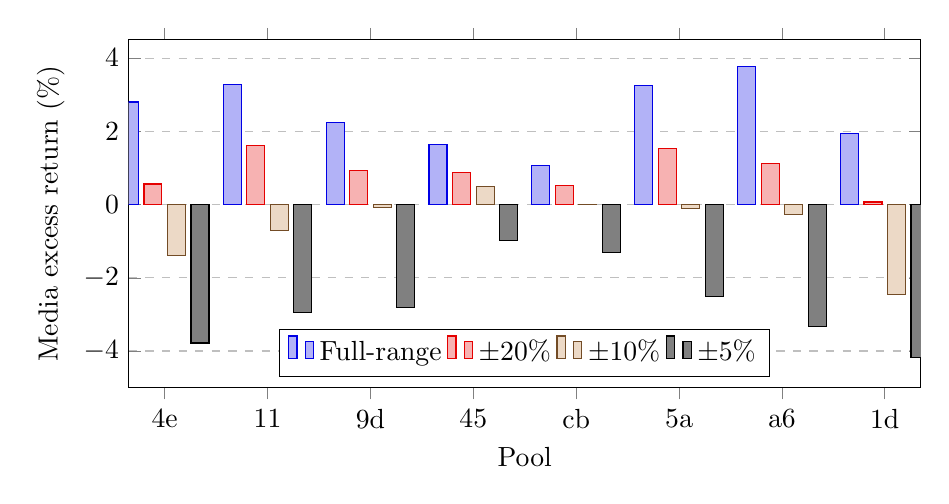
\begin{tikzpicture}
\begin{axis}[
    ybar,
    bar width=6.5pt,
    width=0.96\textwidth,
    height=6cm,
    ymin=-5.0,
    ymax=4.5,
    ylabel={Media excess return (\%)},
    symbolic x coords={4e,11,9d,45,cb,5a,a6,1d},
    xtick=data,
    xlabel={Pool},
    legend style={at={(0.5,0.17)}, anchor=north, legend columns=4},
    ymajorgrids=true,
    grid style=dashed,
    enlarge x limits=0.05,
]
\addplot coordinates {(4e,2.80) (11,3.28) (9d,2.24) (45,1.65) (cb,1.06) (5a,3.24) (a6,3.77) (1d,1.95)};
\addplot coordinates {(4e,0.56) (11,1.61) (9d,0.92) (45,0.88) (cb,0.52) (5a,1.54) (a6,1.12) (1d,0.07)};
\addplot coordinates {(4e,-1.39) (11,-0.71) (9d,-0.07) (45,0.50) (cb,-0.01) (5a,-0.12) (a6,-0.28) (1d,-2.46)};
\addplot coordinates {(4e,-3.78) (11,-2.95) (9d,-2.80) (45,-0.98) (cb,-1.31) (5a,-2.51) (a6,-3.34) (1d,-4.18)};
\legend{Full-range,$\pm 20\%$,$\pm 10\%$,$\pm 5\%$}
\end{axis}
\end{tikzpicture}
\caption{Median monthly net LP excess return over HODL under stylized passive Uniswap v3 strategies by pool and band width.}
\label{fig:stylized_v3_median_excess}
\end{figure*}


\subsubsection{Same-sample proxy alignment under passive range concentration}
\label{subsubsec:proxy_vs_realized}

{We next compare the pool ranking implied by the proxy layer to the realized ordering induced by the stylized passive Uniswap v3 simulation. Net90 is the tail-adjusted screening score defined in Section~\ref{sec:metrics}. It combines fee yield with a 10th-percentile proxy IL downside term. Here, Net90 is computed over the same pool-month sample used in the v3 simulations. This comparison is a same-sample alignment diagnostic rather than a predictive backtest. It assesses whether the proxy metric captures the cross-sectional pool attractiveness observed in the realized passive-v3 strategies.}

{Table~\ref{tab:proxy_vs_realized_ranks} presents the same-sample Net90 rank together with the realized ranks under full-range, $\pm20\%$, $\pm10\%$, and $\pm5\%$ bands. The realized ranks are based on median monthly excess return relative to HODL. Fig.~\ref{fig:concentration_breakdown} summarizes the alignment using Spearman rank correlation, a rank-based measure of whether two orderings place pools in a similar order. 
Values near \(1\) indicate strong agreement, while negative values indicate reversed rankings.
The results show strong agreement under broad passive exposure. The correlation is 0.952 under full-range exposure and remains high at 0.786 under the $\pm20\%$ band. These results suggest that the proxy layer captures pool-level fee and inventory-risk tradeoffs that remain relevant when range constraints are weak.}

{The ranking relationship changes under tighter passive ranges. The Spearman correlation falls to $-0.310$ under both the $\pm10\%$ and $\pm5\%$ bands. The rank table shows that this reversal is driven mainly by the WBTC/WETH pools. Pool 45 has Net90 rank 7, but becomes the top-ranked pool under both the $\pm10\%$ and $\pm5\%$ bands. Pool cb has Net90 rank 8, but rises to realized rank 2 under both tighter bands. In contrast, pools that rank highly under Net90, such as a6, 5a, and 11, move to lower realized positions once the range becomes tight.}

{This deterioration is consistent with the active-share patterns reported in Table~\ref{tab:stylized_v3_results}. As ranges narrow, positions spend less time in range, which makes realized outcomes more dependent on range mechanics rather than only on the pool-level fee and inventory-risk tradeoff summarized by Net90. At that point, realized performance depends more on the realized price path, the timing of range exits, and the inventory composition accumulated while the position is inactive.}

{The comparison clarifies the scope of the proxy layer. 
Net90 is informative as a pool-level screening metric for full-range and wide passive LP strategies. 
It is less informative under tight concentration because it does not measure whether a passive position remains active. 
Thus, poor alignment under tight bands does not make the proxy layer meaningless. 
Rather, it shows that once range inactivity dominates, a pool-level divergence-and-fee proxy is no longer sufficient. 
Narrow passive Uniswap v3 ranges introduce a separate range-risk channel that can dominate the original pool-level ranking.}

\begin{figure*}[t]
\centering
\footnotesize

\begin{minipage}[t]{0.60\textwidth}
\vspace{0pt}
\centering
\begin{tabular}{lccccc}
\toprule
Pool & Net90 rank & Full-range & $\pm20\%$ & $\pm10\%$ & $\pm5\%$ \\
\midrule
a6 & 1 & 1 & 3 & 5 & 6 \\
5a & 2 & 3 & 2 & 4 & 3 \\
11 & 3 & 2 & 1 & 6 & 5 \\
9d & 4 & 5 & 4 & 3 & 4 \\
4e & 5 & 4 & 6 & 7 & 7 \\
1d & 6 & 6 & 8 & 8 & 8 \\
45 & 7 & 7 & 5 & 1 & 1 \\
cb & 8 & 8 & 7 & 2 & 2 \\
\bottomrule
\end{tabular}
\captionof{table}{Same-sample Net90 ranks versus realized passive-v3 ranks.}
\label{tab:proxy_vs_realized_ranks}
\end{minipage}
\hfill
\begin{minipage}[t]{0.36\textwidth}
\vspace{0pt}
\centering
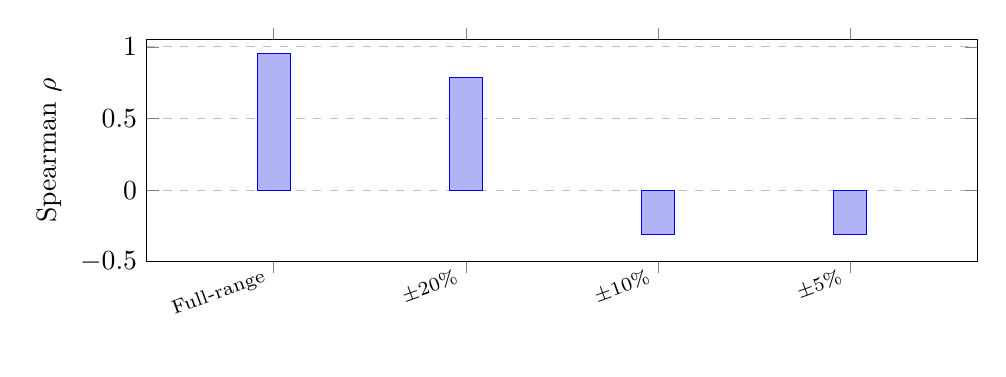
\begin{tikzpicture}
\begin{axis}[
    ybar,
    bar width=12pt,
    width=\textwidth,
    height=4.4cm,
    ymin=-0.50,
    ymax=1.05,
    ylabel={Spearman $\rho$},
    symbolic x coords={Full-range,$\pm20\%$,$\pm10\%$,$\pm5\%$},
    xtick=data,
    xticklabel style={font=\scriptsize, rotate=20, anchor=east},
    ymajorgrids=true,
    grid style=dashed,
    enlarge x limits=0.22,
]
\addplot coordinates {
    (Full-range,0.952)
    ($\pm20\%$,0.786)
    ($\pm10\%$,-0.310)
    ($\pm5\%$,-0.310)
};
\end{axis}
\end{tikzpicture}
\caption{Spearman rank correlation between same-sample Net90 ranks and realized passive-v3 ranks.}
\label{fig:concentration_breakdown}
\end{minipage}

\end{figure*}

{Taken together, the empirical results clarify both the usefulness and the limitation of the proxy framework. The full-range proxy metrics identify persistent cross-pool differences in divergence risk and fee compensation, and their rankings align closely with realized outcomes under full-range and wide passive v3 exposure. However, the alignment deteriorates under tight passive concentration, where range inactivity and path-dependent inventory effects become dominant. The proxy layer should therefore be interpreted as a pool-screening tool for broad or moderately concentrated passive exposure, not as a complete model of optimized Uniswap v3 range selection.
}


\section{Discussion: Scope and Implications of Proxy-Based LP Screening}
\label{sec:discussion}

The empirical analysis positions the proposed metrics as a general LP screening layer rather than a Uniswap-v3-specific strategy model. 
We now highlight three implications. 
First, the proxy metrics provide an ex-ante view of fee compensation, pair-level divergence risk, downside exposure, and persistence. 
Second, pool comparison should focus on fee velocity rather than fee tier alone. 
Finally, the passive-v3 simulations show how pool screening can be combined with protocol-specific strategy analysis when range mechanics affect realized LP outcomes.

\subsection{From Proxy Metrics to Pool Screening}

The proxy metrics capture distinct dimensions of the LP screening problem. 
The IL summaries measure the distribution of price-ratio divergence, the fee-yield summaries measure compensation for bearing that divergence, and the half-life statistic measures the persistence of deviations once they occur. 
Together, these quantities provide a screening view that is richer than ranking pools by fee tier, raw volume, or individual-token volatility alone.

The main empirical pattern is that divergence risk is driven by relative price dynamics rather than by the volatility of either token in isolation. 
In this sample, WBTC/WETH pools exhibit lower proxy IL because the two assets co-move, while stable--volatile pools expose the LP directly to the volatile asset's movement against the stable numeraire. 
This does not imply that correlated pools are Inherently superior, since realized profitability also depends on fee velocity, liquidity depth, and tail events. 
It does imply that pair-level co-movement is a first-order screening variable across LP environments.

The distributional metrics are also important because average outcomes can hide adverse episodes. 
Pools with similar mean proxy IL may differ substantially in their downside bounds, and pools with attractive median behavior may still experience severe tail losses during dislocations. 
This motivates using downside-aware metrics, such as the 10th-percentile proxy IL term in Net90, rather than relying only on average IL or average fee yield.

Finally, the persistence estimates show that divergence episodes can last long enough to matter for LP decisions. 
Across the analyzed pools, relative-price shocks often decay over several weeks rather than within a few days. 
This makes horizon choice important, since shorter holding periods are more likely to end while a divergence episode is still unresolved. 
Although the AR(1) half-lives do not fully describe the price process, they provide a useful indication of how quickly divergence risk tends to dissipate in each pool.

\subsection{Fee Velocity Rather Than Fee Tier}

The empirical results show why fee tier alone is not enough to assess LP compensation. 
A lower-fee pool can outperform a higher-fee pool when its turnover is sufficiently larger. 
For example, before accounting for IL, a 0.05\% pool must generate more than six times the turnover of a 0.30\% pool to produce higher fee yield. 
This makes fee velocity, rather than raw fee tier or raw trading volume, the relevant object for pool screening.

The relationship can be approximated by
\[
y^{\mathrm{fee}}_t
\approx
\mathrm{FeeTier}
\cdot
\frac{\mathrm{Volume}_t}{\mathrm{TVL}_t}.
\]
This expression separates unit fee margin from capital turnover. 
High-volume pools may still be unattractive if the turnover advantage does not compensate for the lower fee tier. 
Conversely, high-fee pools may underperform when liquidity is large and turnover is low.

This observation motivates the fee component of Net90. 
Fee income is only one side of the LP tradeoff: A pool with high fee velocity may still be unattractive if its relative price is unstable, while a lower-fee pool with high turnover and mild divergence can offer a better risk-adjusted profile. 
Pool selection should therefore account for both fee velocity and downside proxy IL, rather than treating fees or IL in isolation.

\subsection{Implications for LP Strategy Design}

The passive-v3 simulations show how far the proxy framework can be taken in concentrated-liquidity settings. 
Under full-range and wide passive bands, the Net90 ranking remains closely aligned with realized excess returns. 
This suggests that the proxy layer captures pool-level fee and divergence tradeoffs that still matter when range constraints are weak. 
In these cases, the main decision is which pair and fee tier to provide liquidity to, and the full-range proxy remains informative.

The picture changes under tighter passive bands. 
As the range narrows, the position spends fewer days in range, which directly reduces fee accrual. 
At the same time, exiting the range leaves the LP with one-sided inventory exposure, so realized outcomes become more sensitive to the timing and direction of price movements. 
These effects are specific to the chosen range and are not captured by full-range proxy IL. 
The deterioration in rank alignment under tighter bands therefore, reflects a range-inactivity channel: Once positions are inactive for a large share of the holding period, pool-level screening is no longer enough on its own.

This leads naturally to a two-stage view of LP strategy design. 
The proposed metrics can first be used to identify candidate pools with attractive fee-divergence tradeoffs. 
A second stage can then evaluate the protocol-specific choices that determine realized performance after the pool is selected. 
For Uniswap v3, this means range selection, active share, rebalancing frequency, gas costs, slippage, and path-dependent inventory exposure. 
For other AMM designs, the relevant second-stage variables may include bonding-curve shape, pool weights, amplification parameters, or multi-asset inventory exposure.

These results position the framework as a screening tool rather than a complete LP strategy model. 
The paper does not claim that full-range CPMM IL exactly describes every LP position, or that the Uniswap v3 simulation covers all possible concentrated-liquidity strategies. 
Rather, it proposes a general statistical screening layer for LP risk and return, and uses Uniswap v3 as a demanding setting in which the strengths and limits of proxy-based screening can be observed. 
The resulting framework is meant to complement more detailed protocol-specific LP strategy models, not replace them.

\section{Conclusion}
\label{sec:conclusion}
In this paper, we study IL and LP pool-screening metrics in Uniswap v3 to provide LPs with a practical, data-driven way to quantify IL risk and compare pools beyond simple fee-tier heuristics. 
Using multi-year pool data, we show that net outcomes are driven by the interaction of fee generation and divergence risk, motivating simple selection rules based on distributional IL summaries, tail bounds, and predictability diagnostics. 
The stylized passive-v3 analysis shows that these proxy metrics remain informative for full-range and wide passive exposure, but become less sufficient under tight concentration, where range inactivity can dominate.
Future work will extend the analysis to a broader pool universe across additional DeFi platforms and develop protocol-specific range-selection and adaptive fee policies that adjust to time-varying IL risk.

% In this paper, we study IL in Uniswap v3 to provide LPs with a practical, data-driven way to quantify IL risk and compare pools beyond simple fee-tier heuristics. 
% Using multi-year pool data, we show that net outcomes are driven by the interaction of fee generation and divergence risk, motivating simple selection rules based on distributional IL summaries, tail bounds, and predictability diagnostics. 
% Future work will extend the analysis to a broader pool universe across additional DeFi platforms and develop an adaptive fee policy that adjusts fees using rolling correlation and realized net performance to better match time-varying IL risk.

% \section*{Acknowledgments}
% \noindent\textbf{AI content disclosure.} The paper used OpenAI, Gemini, and Grammarly for language editing (grammar, clarity, and \LaTeX{}/formatting suggestions). The authors are responsible for the technical content and for verifying the final manuscript.


\bibliography{references}

\end{document}